% chktex 46

% Author:   Giorgio Färber
% Date:     2024-04

\documentclass[11pt, titlepage]{article}

%% Import all packages %%

% Language and Fonts
\usepackage[utf8]{inputenc}
\usepackage[ngerman]{babel}
\usepackage{csquotes}
\usepackage[T1]{fontenc}
% \usepackage{fancyhdr}
% \pagestyle{fancy}



% Page formatting
\usepackage{geometry}
\usepackage{scrlayer-scrpage}
\usepackage{textcmds}
\usepackage{lastpage}
\geometry{
    paper=a4paper,
    inner=2.0cm, % Inner margin
    outer=2.0cm, % Outer margin
    bindingoffset=0.0cm, % Binding offset
    top=2.0cm, % Top margin
    bottom=2.0cm, % Bottom margin
}

% Maths
\usepackage{amsmath}
\usepackage{eqparbox}

% Allow Python
% \usepackage{datatool, filecontents}
% \input{Latex/special-pages/result_values}



% SI unit Syntax
\usepackage{siunitx}

% Tables and Graphics
\usepackage{graphicx}
\usepackage{booktabs}

% Multiline Comments
\usepackage{comment}

% Code Snippets
\usepackage{listings}
\usepackage{xcolor}
    % Define custom colors for syntax highlighting
    \definecolor{mygreen}{rgb}{0,0.6,0}
    \definecolor{mygray}{rgb}{0.5,0.5,0.5}
    \definecolor{mymauve}{rgb}{0.58,0,0.82}

    % Configure listings settings
    \lstset{ %
    backgroundcolor=\color{white},   % Choose the background color
    basicstyle=\ttfamily\footnotesize, % Set the font style
    breaklines=true,                 % Automatic line breaking
    commentstyle=\color{mygreen},    % Style for comments
    keywordstyle=\color{blue},       % Style for keywords
    stringstyle=\color{mymauve},     % Style for strings
    numberstyle=\tiny\color{mygray}, % Style for line numbers
    numbers=left,                    % Line numbers on the left
    numbersep=5pt,                   % Space between line numbers and code
    frame=single,                    % Frame around the code
    language=[x86masm]Assembler,     % Set the language to Assembly
    xleftmargin=30pt,                    % Left margin
    xrightmargin=30pt,                   % Right margin
    aboveskip=10pt,                      % Space above the listing
    belowskip=10pt,                       % Space below the listing
    }

% Bibliography
\usepackage[
   natbib=true,
   style=numeric,
   sorting=none
   ]
   {biblatex}
% \usepackage{biblatex}
\addbibresource{Sources.bib}
\usepackage{pdfpages}

% Citation
\usepackage[
    left = \flqq{},%
    right = \frqq{},%
    leftsub = \flq{},%
    rightsub = \frq{} %
]{dirtytalk}

% Glossary
% \usepackage{glossaries}
% \usepackage[acronym, toc, nonumberlist]{glossaries}
% \usepackage[nonumberlist, nopostdot, noindex]{glossaries}
% \usepackage[automake]{glossaries-extra}

% \newglossary[tlg]{common}{tld}{tdn}{Glossary}
% \newglossary[slg]{symb}{syi}{syg}{List of Symbols}
% todo: fix the tool glossary!!!
% \newglossary[atg]{tools}{atd}{ato}{Auxiliary Tools Glossary}
% \makeglossaries

% \input{Latex/special-pages/glossary}
% \input{Latex/special-pages/list_of_symbols}
% \input{Latex/special-pages/list_of_tools}

% \setcounter{tocdepth}{2}


% Hyperref
\usepackage{hyperref}
% Define the color of the links
\hypersetup{
    colorlinks=false,
    linkcolor=black,
    filecolor=magenta,
    urlcolor=blue,
}

%%* End packages section *%%

%%* Pagestyle and Commands *%%
\newcommand{\HRule}[1]{\rule{\linewidth}{#1}}
\newcommand{\Pg}{\par\bigskip}

% \setlist[itemize,1]{after=\vskip2\baselineskip}
\linespread{1.25}

\clearpairofpagestyles
\pagestyle{scrheadings}
\pagenumbering{arabic}

% \pagestyle{plain}
\ihead{Biomechanik}
\ohead{Brugger, Färber, Gerg, Münzer}
% \cfoot{\thepage}
% \cfoot[\pagemark]{\pagemark{} of \pageref{LastPage}}
\cfoot[\thepage]% for pagestyle `scrplain`
     {\thepage}% for pagestyle `scrheading`

\setlength{\marginparwidth}{2cm}
\setlength\headheight{17pt}
\setlength{\parindent}{0pt}

% When should the counter be reset?
\numberwithin{figure}{section}
\numberwithin{table}{section}
\numberwithin{equation}{section}

%%* End of SETUP *%%


\begin{document}

%* Title Page *%

\begin{titlepage}
   \begin{center}
       \vspace*{1cm}

       \Huge
       \textbf{
         ANALYSE: ASYMMETRISCHE MUSKELBELASTUNG BEI KNIEBEUGEN VOR UND NACH AUSGLEICHSÜBUNGEN
       }

       \vspace{0.5cm}
       \LARGE

       \vspace{1.5cm}

       \textbf{Biomechanik Projekt}
       \vfill

       \textbf{Franziska Brugger, Giorgio Färber, Maximilian Gerg, Felix Münzer}
       \vfill

       \begin{center}
         
\includegraphics[width=0.7\textwidth]{img/hm-logo.jpg}
         \\
         \normalsize
       \end{center}


       \vfill

       % \vspace{0.8cm}

       \Large


       \vspace{0.8cm}
       \centering

       15. Januar 2025



   \end{center}
 \end{titlepage}
\setcounter{page}{2}

%* Abstract *%
\section*{\centering Abstrakt}
Dieses Projekt untersucht asymmetrische Muskelbelastungen beim Ausführen von Kniebeugen vor und nach spezifischen Ausgleichsübungen. 
Ziel war es, potenzielle Dysbalancen zwischen der linken und rechten Körperseite zu identifizieren und durch gezielte Übungen zu reduzieren. 
Die Messungen erfolgten sowohl mit Wägezellen als auch mittels Elektromyographie (EMG). 
Dabei zeigte sich, dass bei allen Probanden Asymmetrien in der Gewichtsverteilung und Muskelaktivierung vorlagen. 
Nach einem vierwöchigen Training mit Ausgleichsübungen konnte eine Verbesserung der Symmetrie festgestellt werden. 
Die Ergebnisse verdeutlichen, dass gezielte Ausgleichsübungen effektiv Dysbalancen reduzieren können, was sowohl im Alltag als auch im sportlichen Bereich von Bedeutung ist.
\clearpage

% Header and footer information
%\setlength\headheight{15pt}
%\fancyhead[L]{Analyse: asymetrische  Muskelbelastung im Kraftsport (Liegestützen, Kniebeugen, Klimmzüge) und Ausgleichstraining\\}
%\fancyhead[R]{Franziska Brugger, Giorgio Faerber, Maximilian Gerg, Felix Muenzer}
% \fancyfoot[C]{\thepage}
% \setlength {\marginparwidth }{2cm}


\tableofcontents %Hier wird das Inhaltsverzeichnis eingefügt%
\clearpage

\listoffigures
\listoftables
\clearpage
% \newpage

\setcounter{section}{0}

%%%%%%%%%%%%%%%%%%
%HIER GEHT ES LOS%
%%%%%%%%%%%%%%%%%%


\section{Motivation}

Ambidextrie beschreibt die Fähigkeit mit beiden Händen gleich geschickt zu sein \cite{wissen.de}. Da die meisten  Menschen nicht ambidextr sind, haben sie eine stärkere und eine schwächere Seite. Das ist beim Schreiben oder Malen nicht weiter problematisch. Werden aber bei Belastung wie körperlicher Arbeit oder beim Sport Muskeln unterschiedlich stark belastet, kann das zu Fehlhaltungen und Schmerzen führen. Dadurch können Gelenke ungünstig belastet werden, was zu Gelenkverschleiß führen kann.\\
Muskuläre Dysbalancen können verschiedene Ursachen haben. \\
\\
 \subsection{Fehlhaltung im Alltag}
 Personen die im Alltag überwiegend sitzen nehmen häufig eine Fehlhaltung ein, was zu einer Dysbalance zwischen Brust- und oberer Rückenmuskulatur führen kann. Auch werden viele anstrengende Aufgaben, wie das Tragen von schweren Taschen oder das Öffnen von Marmeladengläsern, meist mit der stärkeren Hand erledigt. Dadurch wird diese Seite sträker und beweglicher, was zu Schulterproblemen führen kann.

 \subsection{Fehlhaltung nach Verletzungen}
 Durch Verletzungen können kompensierende Fehlhaltungen entstehen. Ein verletztes Knie kann zum Beispiel dazu führen, dass Menschen mit der verletzten Seite weniger stark auftreten. Das unverletzte Bein wird dadurch stärker beansprucht, wodurch das gesunde Bein stärker beansprucht wird und die Muskeln am verletzten Knie sogar weiter abnehmen.

 \subsection{Falsches Training}
Werden beim Kraftsport Übungen fehlerhaft ausgeführt, gleicht der Körper das ungleiche Kräfteverhältnis meist unbemerkt aus.

\begin{quote}
Steht das Becken nach rechts schief, dreht der Brustwirbel den Oberkörper nach links ein, das Kopfgelenk neigt den Kopf wieder nach rechts und so weiter – bei Sportlern findet meistens eine Art Kettenreaktion von unten nach oben statt. Dann sind die Augen wieder horizontal und man merkt nicht, dass man überhaupt eine Fehlhaltung eingenommen hat" \cite{MensHealth}
\end{quote}
Bei Kniebeugen kann es dann zum Beispiel passieren, dass sich der Sportler auf eine Seite lehnt und dadurch das kräftigere Bein stärker beansprucht als das ohnehin bereits schwächere Bein. \\
\\



\section{Messinstrumente}
% % Technische Umsetzung Wägezelle
% % EMG-Messung
\subsection{Wägezelle}
%todo: Quellen?
Wägezellen messen mechanische Verformungen.
Wird auf eine Wägezelle eine Gewichtskraft \mbox{$F = m \cdot g \: [\frac{kg \cdot m}{s^2}]$} (m = aufgebrachte Masse und $g = 9.81 \: \frac{m}{s^2}$)  aufgebracht, verformt sich diese unter der Krafteinwirkung.
Auf der Wägezelle sind Dehnungsmessstreifen aufgebracht, deren Widerstand sich bei einer Verformung ändert.
Die Dehnungsmessstreifen sind in einer Wheatstone-Brücke verschaltet, die die Widerstandsänderung in eine Spannungsänderung umwandelt, die meist nur im Bereich weniger Millivolt liegt.
Diese Spannungsänderung ist proportional zur aufgebrachten Gewichtskraft.
Unten dargestellt in \autoref{fig:CAD-Darstellung-Waegezelle} ist der Aufbau einer Wägezelle als CAD-Modell. \\
\begin{figure}[h!]
    \centering
    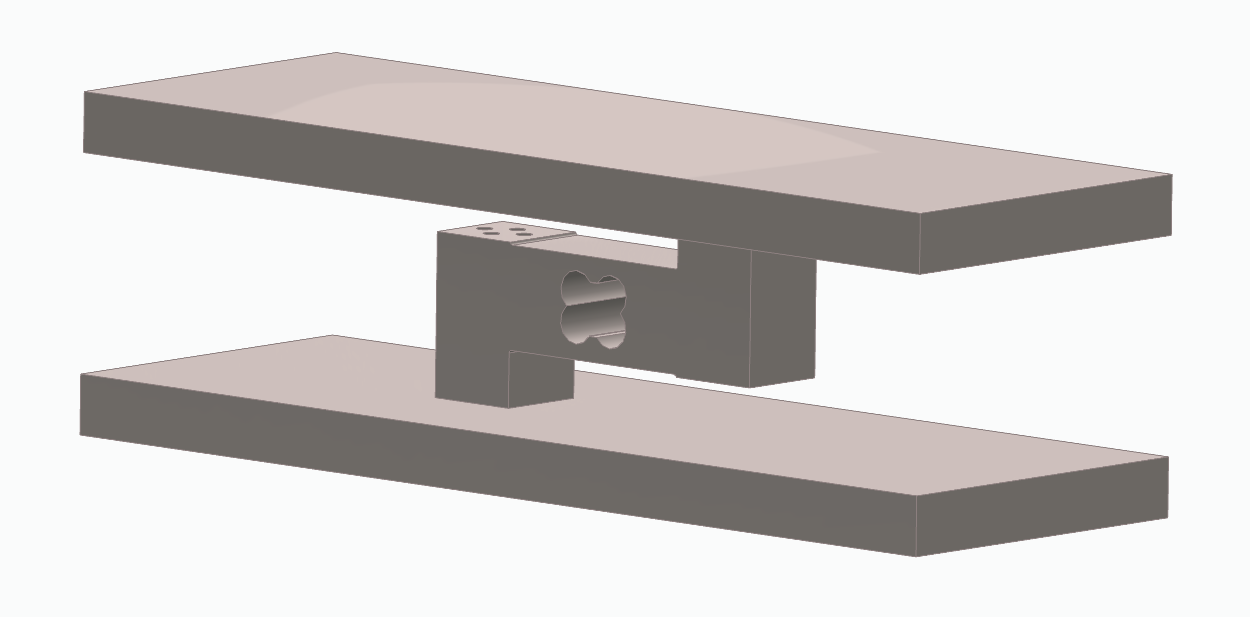
\includegraphics[width=0.6\textwidth]{img/CAD_Waegezelle.png}
    \caption{CAD Darstellung Wägezelle}
    \label{fig:CAD-Darstellung-Waegezelle}
\end{figure}

% \begin{figure}[h!]
%    \centering
%    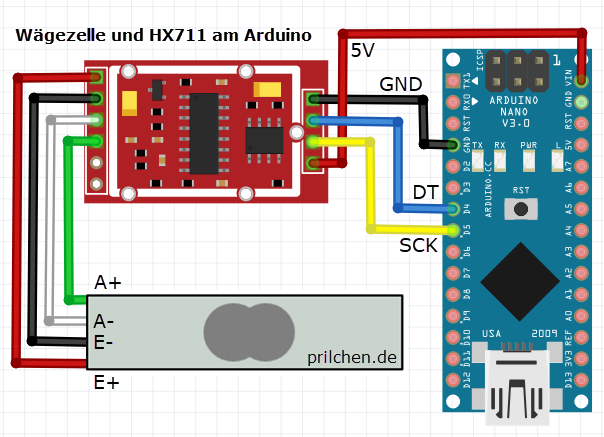
\includegraphics[width=0.6\textwidth]{img/waegezelle_verschaltung.png}
%    \caption{HX711 Schaltung mit Arduino Nano \cite{prilchen}}
%    \label{fig:HX711-Nano-Schaltung}
% \end{figure}
% Um die Signale der Wägezelle an den HX711 weiterzugeben und die Signale des HX711 mit dem Arduino Nano verarbeiten und die Daten lesbar darzustellen, müssen die drei Komponenten miteinander verschaltet werden und korrekt kommunizieren.
% Dies wird mit der in \autoref{Gesamtaufbau-waegezelle-mit-Arduino-Nano} dargestellten Schaltung erreicht.\\
% Zuerst wird die Wägezelle an eine 5 V Gleichstromquelle angeschlossen und dann mit dem HX711 verbunden.
% Wodurch die Wägezelle die analogen Signale an den HX711 weitergeben kann.
% Der HX711 wandelt sie dann in ein digitales Signal und gibt dieses an den Arduino Nano weiter.
% Der VCC-Pin HX711 wird mit dem 5V-Pin des Arduino Nano verbunden.
% Der GND-Pin mit dem GND-Pin des Ardiunos.
% Der DT-Pin ist der Datenausgang des HX711 und wird mit irgendeinem der Digital-Pins des Nanos verbunden, genauso wie der SCK-Pin, z.B. $DT-Pin -> D3-Pin$ und $SCK-Pin -> D2-Pin$.
% Der SCK-Pin oder serial-clock-Pin steuert die Übertragung des Signals des DT-Pins.
% Der Arduino gibt auf dem SCK-Pin den Takt vor, mit dem der HX711 die Daten an den Mikrocontroller sendet.
% Der Ardiuno setzt den SCK-Pin auf high und dann wieder auf low. Dieser Wechsel, vom Ende eines low-Signals zu einem high- und wieder einem low-Signal ist ein Takt.
% Der HX711 sendet dann pro Takt ein Bit, also einen low-Puls für 0 und einen high-Puls für 1.
% Der Arduino-Nano wird dann an einen Computer angeschlossen.
% In der Arduino IDE können mithilfe der passenden Library und einem Code die Daten ausgelesen und gespeichert werden.
% \\
% \\
% Der auf dem Arduino ausgeführte C-Code liest periodisch den analogen Wert des HX711 aus. Zunächst muss der Sensor initialisiert werden. Dies geschieht durch:
% \begin{enumerate}
%     \item \textbf{Angabe eines Kalibrationswertes}: Dieser Wert dient der genauen Gewichtsmessung.
%     \item \textbf{Tara-Einstellung}: Die Waage wird auf 0 kg gesetzt, um sicherzustellen, dass nachfolgende Messungen korrekt sind.
% \end{enumerate}
% Nach der Initialisierung ist die Waage bereit, Messdaten auszugeben.
% \\
% Für die Ausgabe eines Messwerts werden die gemessenen Daten über den Serial-Port übertragen.
% Dabei wird angegeben, ob die Messung von der linken oder rechten Waage stammt.
% Die Ausgabe erfolgt beispielsweise wie folgt:
% \begin{center}
%     \texttt{Gewicht rechts [kg]: -0.00118}  \\
%     \texttt{Gewicht links [kg]: -0.00321} \\
%     \texttt{Gewicht rechts [kg]: -0.00118} \\
%     \texttt{Gewicht links [kg]: -0.00223} \\
% \end{center}
% Der serielle Monitor verarbeitet die Ausgabe des Arduinos und ergänzt jeden Messwert mit einem Zeitstempel, der den Zeitpunkt angibt, zu dem der Messwert den Computer erreicht. Dadurch wird es möglich, die seriellen Daten in Echtzeit als Graph über die Zeit darzustellen, wie in Abbildung \ref{fig:serial_output} veranschaulicht.
% %todo:
% \begin{figure}[h!]
%     \centering
%     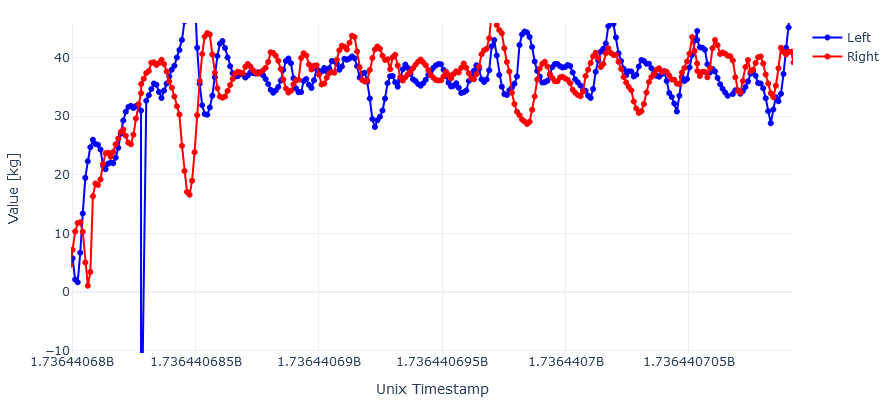
\includegraphics[width=0.7\textwidth]{img/serial_output_example.png} % Screenshot oder Beispiel
%     \caption{Ausgabe der Messdaten mit Python}
%     \label{fig:serial_output}
% \end{figure}
% \\
% Allen Daten werden in einem CSV-Format gespeichert.
% Sie können nun beliebig aufbereitet und analysiert werden.
% Der C Code auf dem Arduino liest periodisch den analogen Wert des HX711 aus, muss dafür aber zuerst initialisiert werden.
% Dazu wird ein Kalibrationswert angegeben und anschließend die Waage auf 0 kg getared.
% Nun ist die Waage initialisiert und bereit, Messdaten auszugeben.
% Soll ein Messwert ausgegeben werden, so werden die Daten an den Serial-Port ausgegeben, mit dem Hinweis, ob der Messwert von links oder rechts stammt.
% \begin{center}
%     Gewicht links: ...  \\
%     Gewicht rechts: ...
% \end{center}
% An dem Serial-Port angekommen werden die Daten von einem zweiten parallel laufenden Python Skript ausgewertet.
% Dabei können die Daten in Echtzeit in einer web App dargestellt werden und werden gleichzeitig aufgezeichnet im CSV-Format.
% \\
% Diese Daten können nun auf verschiedene Art und Weisen mithilfe von Python dargestellt werden.


\subsection{Elektromyographie}

Mit einem EMG kann die elektrische Muskel-Aktivität gemessen werden.
Dazu wird die elektrische Aktivität in einem ruhenden und einem kontrahierten Muskel gemessen. Das Signal entsteht aus dem Aktionspotential der Muskelfasermembran und dem Depolarisations- und Repolarisationsverlauf, der in \autoref{fig:depolarisations-und-repolarisationsverlauf} als Funktion der Zeit dargestellt ist. Im Ruhetonus liegt das Potential zwischen $-80$ und  $-90$ mV.
\begin{figure}[h!]
    \centering
    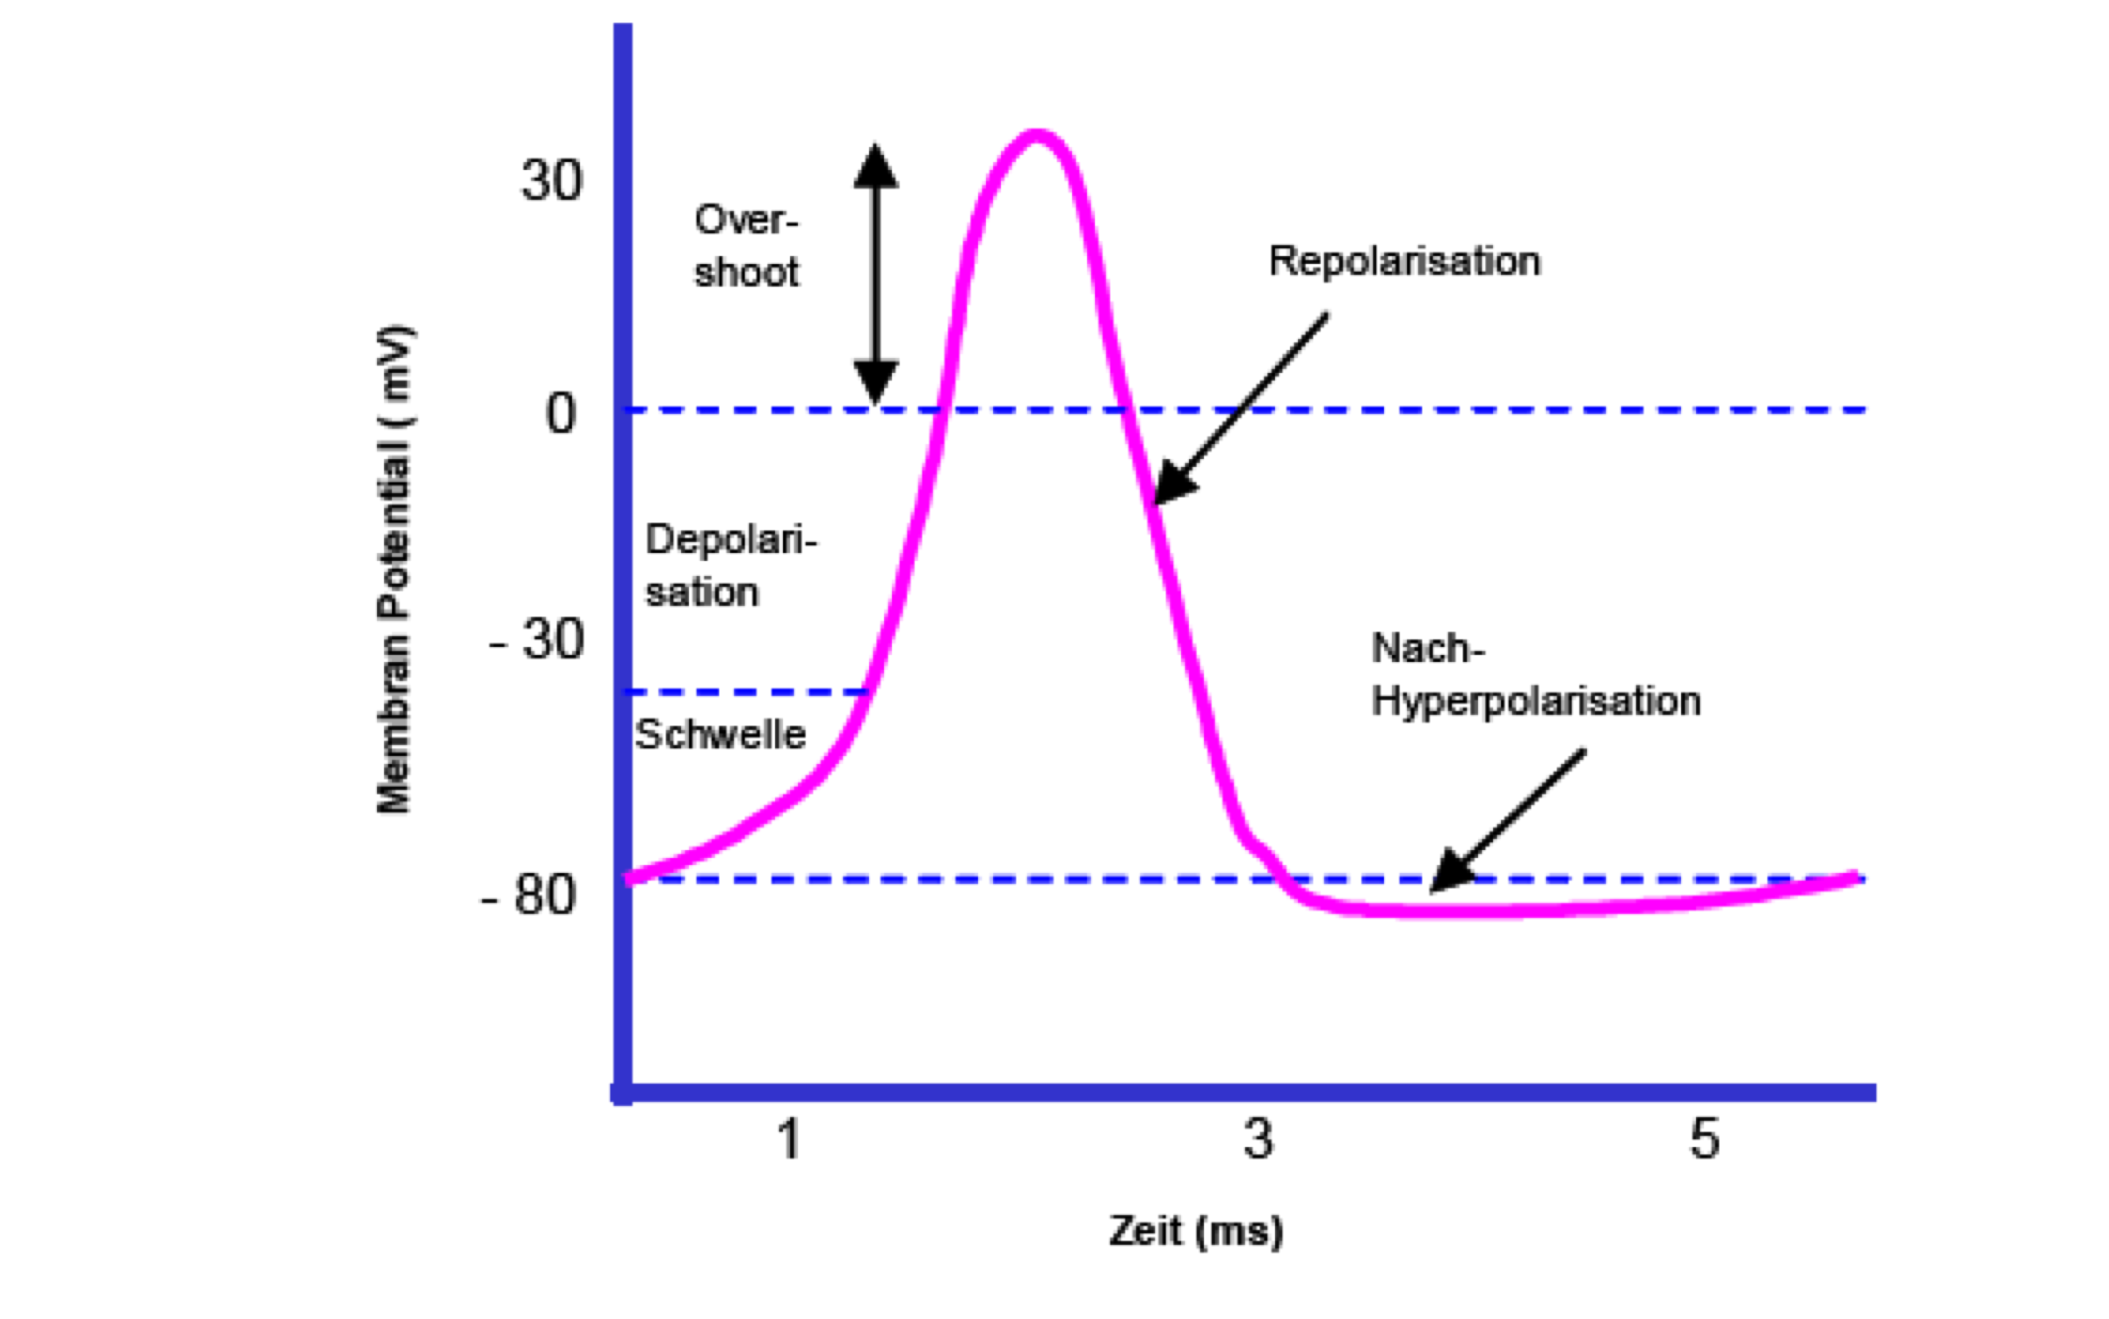
\includegraphics[width=0.8\textwidth]{img/De-Repolarisation.PNG}
    \caption{De- und Repolarisation und Aktionspotential Muskelfasermembran \cite{Vorlesung-Muskulatur-EMG}}
    \label{fig:depolarisations-und-repolarisationsverlauf}
\end{figure}
\\
Eine Muskelkontraktion startet auf Sarkomerebene.
Durch das Zusammenwirken aller Sarkomere wird die Umwandlung von chemischer Energie in mechanische Energie als Kontraktion des Muskels sichtbar.
\\
\\
Ein  Nervenimpuls gelangt als Aktionspotential über das Axon eines Motoneurons zum Axonende. \\
Durch Neurotransmitter die in den postsynaptischen Spalt ausgeschüttet und dann an den Rezeptor der postsynaptischen Membran binden, wird der Prozess der Depolarisation in der Muskelfaser ausgelöst, der auf der linken Seite von  \autoref{fig:depolarisations-und-repolarisationsverlauf} dargestellt ist:\\
\\
Der Rezeptor ist ein Kanal für Kationen, also positiv geladene Ionen wie Natrium-, Calcium- oder Kaliumionen. Wird der Ionenkanal geöffnet, kommt es zum Einfluss von Kationen und zu einer  Depolarisation der Muskelfaser. Wird ein gewisses Schwellenpotential überschritten, öffnen sich spannungsabhängige Natrium-Kanäle, wodurch ein Aktionspotential ausgelöst wird, das als EMG-Signal gemessen werden kann.
In \autoref{fig:depolarisations-und-repolarisationsverlauf} als Schwelle gekennzeichet, ab der die Steigung der Potential-Funktion zunimmt, bis die Funktion bis $+20$ bis $+30$ mV steigt.
Das Aktionenpotential löst nun wiederum die Öffnung von spannungsgesteuerten Calcium-Kanälen aus, wodurch Calcium-Ionen in der Muskelfaser freigesetzt werden. Es kommt zu einer Anhäufung von Calcium-Ionen in der Muskelfaser. Dadurch steigt Calciumkonzentration, was die Kontraktion der Muskelfaser auslöst. \\
Noch bevor der Höhepunkt des Aktionspotentials erreicht ist, werden die Natriumkanäle inaktiv und positiv geladene Kalium strömen aus der Zelle. Das Potential nähert sich nach einer Hyperpolarisationsphase, während der das Pontential unter das Ruhepotential von $-80$ mV fällt, wieder dem Ruhepotential an.
\\
\\
Die EMG-Messung findet in der Hochschule im Labor für Ergonomie statt.
Die Daten werden mithilfe eines Programms von NORAXON ausgelesen und analysiert.




\section{Methodik}
% Projekt Ablauf (Zeitplan)
% Experimentelle Setups + Messung
\subsection{Zeitlicher Ablauf des Gesamtversuchs}
Der Versuch ist so aufgebaut, dass bei der ersten Messung die links- und rechtseitige Belastung der Probanden bei einer Kniebeuge im untrainierten Zustand mit einem EMG gemessen werden. 
Dann haben die Probanden für vier Wochen drei spezifisch ausgewählte Ausgleichsübungen trainiert, die mögliche Ungleichgewichte ausgleichen sollen. 
Nach vier Wochen findet eine zweite Messung statt. Die analog zur ersten Messung abläuft. Bei der zweiten Messung wurden als zusätzliche Messinstrumente zwei Wägezellen eingesetzt. 
Nach der zweiten Messung erfolgt die Auswertung der Ergebnisse. 
Der Ablauf ist in \autoref{fig: Ablauf-gesamtversuch} dargestellt. 
\begin{figure}[h!]
    \centering
    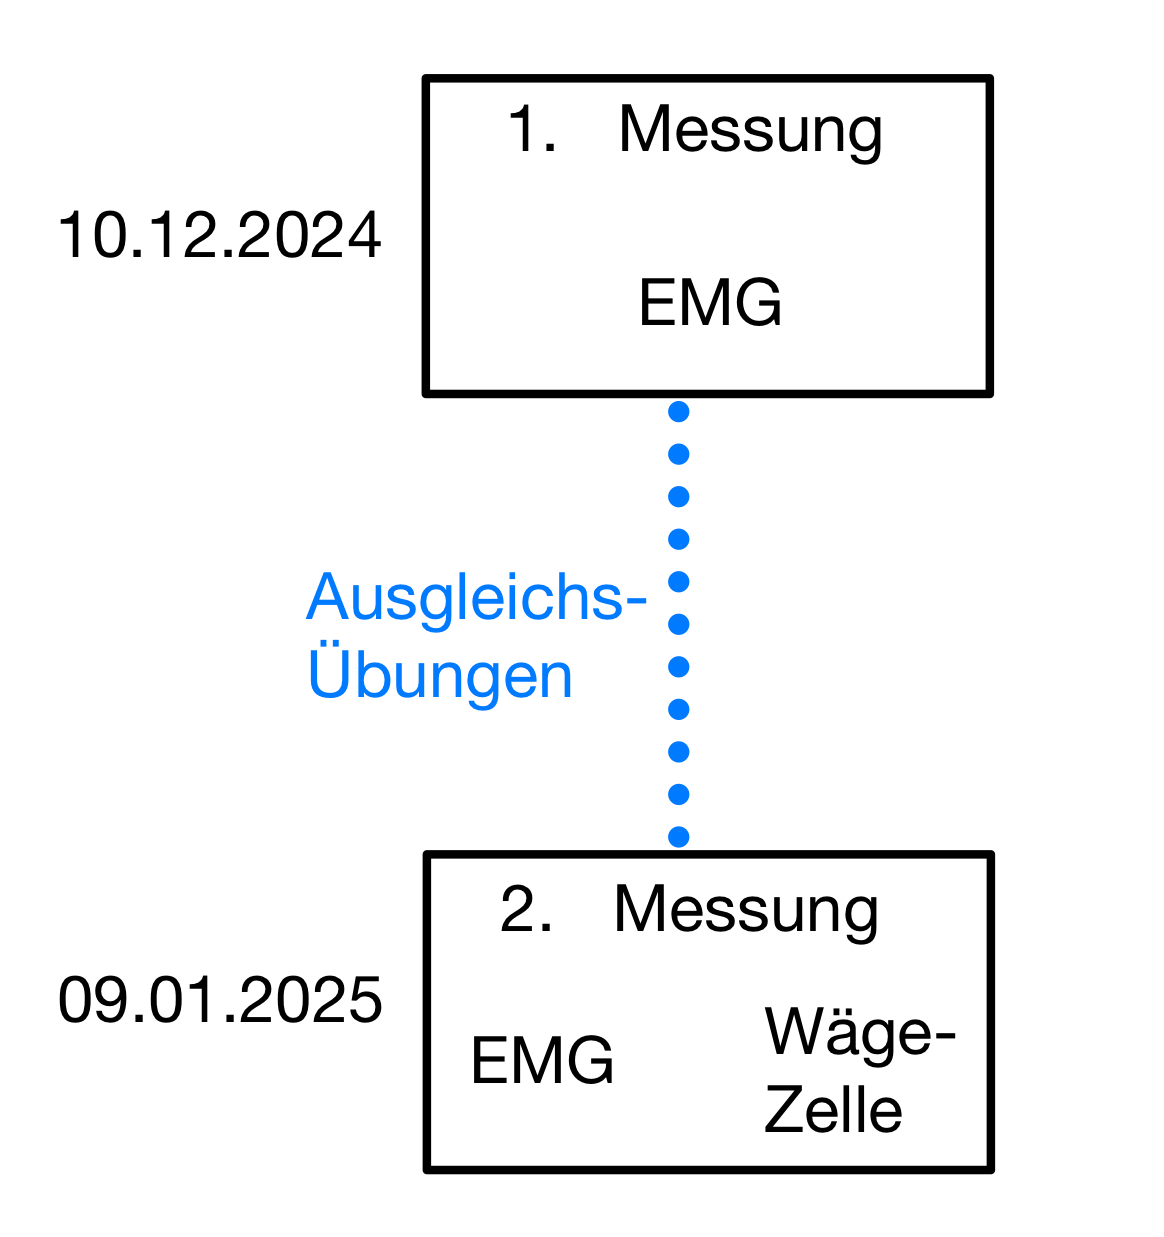
\includegraphics[width=0.4\textwidth]{img/Ablauf-gesamtversuch.jpeg}
    \caption{Zeitlicher Ablauf Versuch}
    \label{fig: Ablauf-gesamtversuch}
\end{figure}
\\
\\ 
\subsection{Wägezelle}
In diesem Versuch werden Wägezellen eingesetzt um etwaige Ungleichgewichte beim Ausführen einer Kniebeuge zu messen.
Hierzu stellt sich der Proband auf zwei Wägezellen und führt eine Kniebeuge aus, die Wägezellen messen während dessen die auf ihnen lastende Gewichtskraft.
Wird eine Seite während der Kniebeuge stärker belastet, sollte die jeweilige Wägezelle einen höhren Wert messen. \\ \\
An die Wägezelle ist der Wägesensor HX711 angeschlossen, der in \autoref{fig:HX711} dargestellt ist.
\begin{figure}[h!]
    \centering
    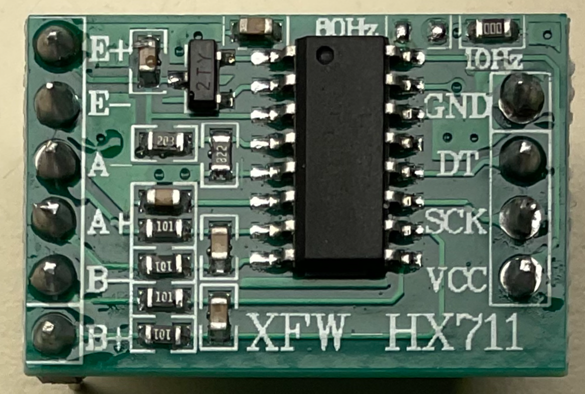
\includegraphics[width=0.3\textwidth]{img/HX711.png}
    \caption{HX711 \cite{prilchen}}
    \label{fig:HX711}
\end{figure}
Der Sensor HX711 ist ein Analog-Digital-Wandler, der die analogen Spannungsänderungen der Wheatstone-Brücke verstärkt und in ein digitales Signal umwandelt.
Dieses digitale Signal kann dann von einem Mikrocontroller verarbeitet werden.
In diesem Projekt wird der Arduino Nano verwendet wie in \autoref{fig:Nano-Pinlayout} dargestellt.
\begin{figure}[h!]
    \centering
    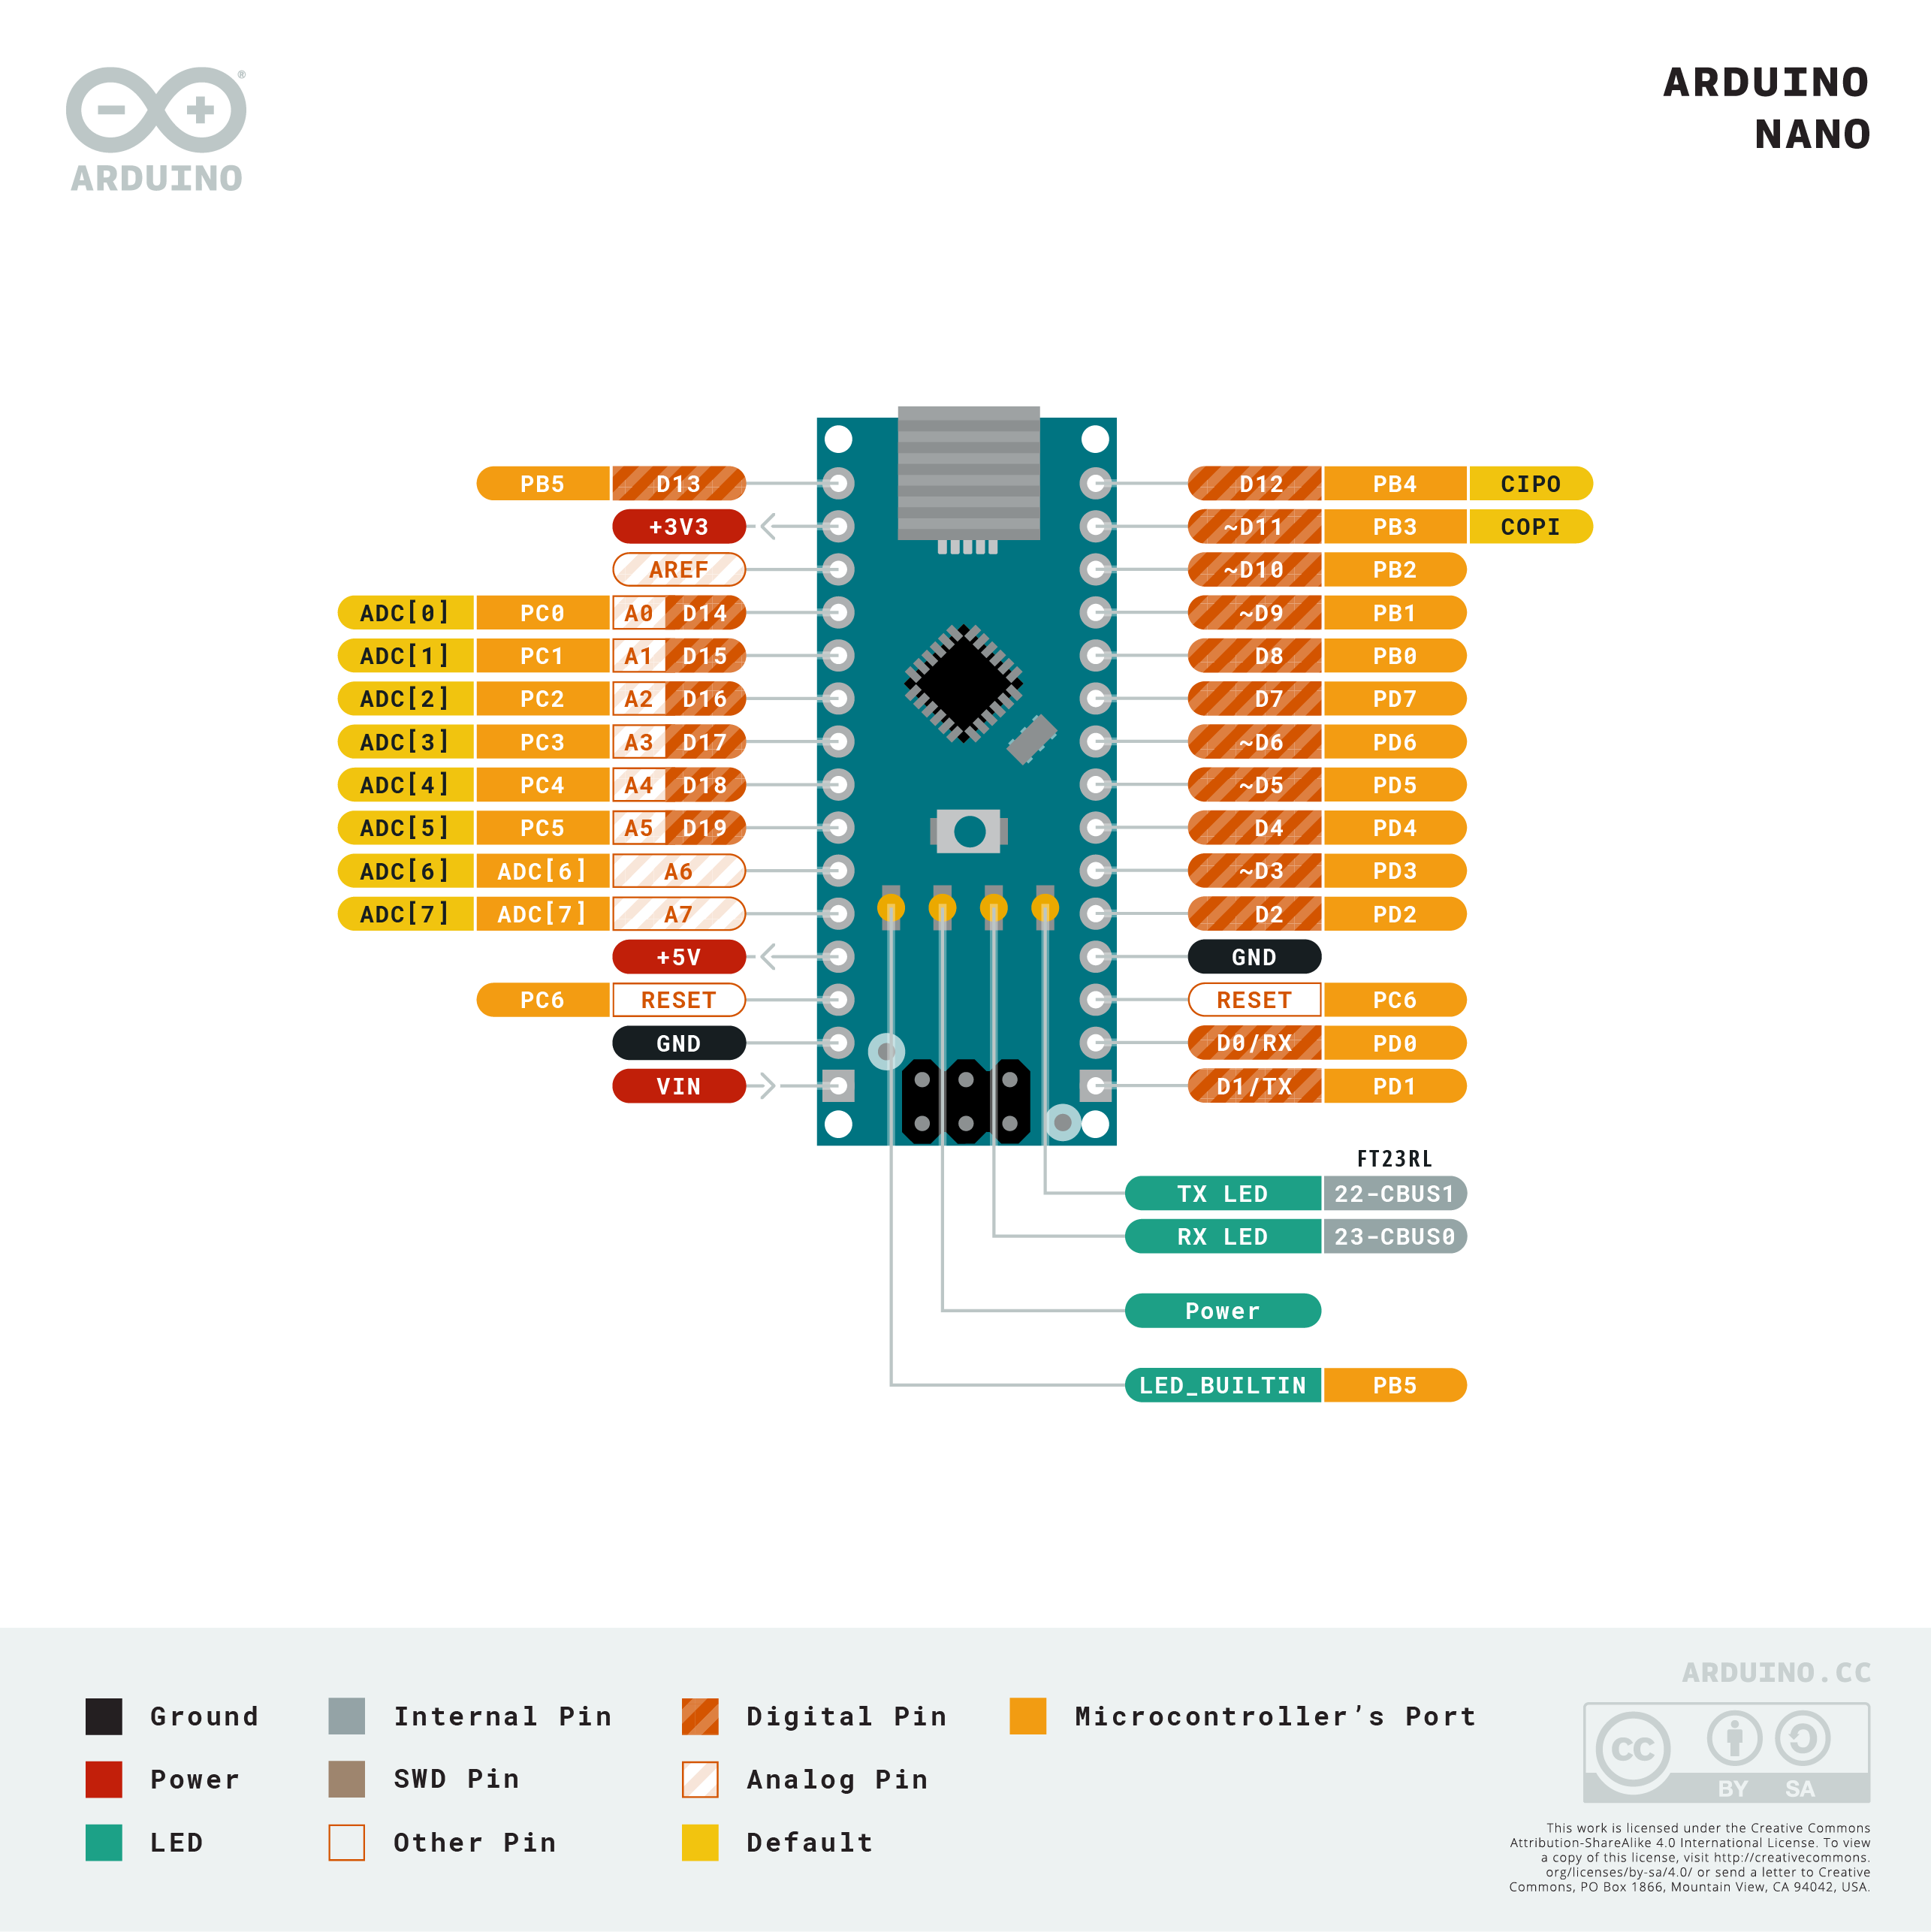
\includegraphics[width=0.8\textwidth]{img/Nano-Pinlayout.png}
    \caption{Nano-Pinlayout \cite{Arduino}}
    \label{fig:Nano-Pinlayout}
\end{figure}
Um den Aufbau verwenden zu können müssen alle Komponenten richtig miteindander verschaltet sein und kommunizieren.
Dafür wird die Wägezelle an eine 5 V Gleichstromquelle angeschlossen und mit dem HX711 verbunden.
Die Wägezelle kann so die analogen Signale an den HX711 weitergeben.
Der HX711 wandelt sie in ein digitales Signal um und gibt dieses an den Arduino Nano weiter.
Der VCC-Pin HX711 wird mit dem 5V-Pin des Arduino Nano verbunden.
Der GND-Pin mit dem GND-Pin des Ardiunos.
Der DT-Pin ist der Datenausgang des HX711 und wird mit irgendeinem der Digital-Pins des Nanos verbunden, genauso wie der SCK-Pin, z.B. $DT-Pin -> D3-Pin$ und $SCK-Pin -> D2-Pin$.
Der SCK-Pin oder serial-clock-Pin steuert die Übertragung des Signals des DT-Pins.
Der Arduino gibt auf dem SCK-Pin den Takt vor, mit dem der HX711 die Daten an den Mikrocontroller sendet.
Der Ardiuno setzt den SCK-Pin auf high und dann wieder auf low.
Dieser Wechsel, vom Ende eines low-Signals zu einem high- und wieder einem low-Signal ist ein Takt.
Der HX711 sendet dann pro Takt ein Bit, also einen low-Puls für 0 und einen high-Puls für 1.
\\
Der Arduino-Nano wird nun an einen Computer angeschlossen.
Wie in \autoref{Gesamtaufbau-waegezelle-mit-Ardiuno-Nano} dargestellt, sind die Wägezellen dann mit den HX711 verbunden und diese wiederum mit einem Arduino-Nano, welcher selber mit einem Computer verbunden ist.
\begin{figure}[h!]
    \centering
    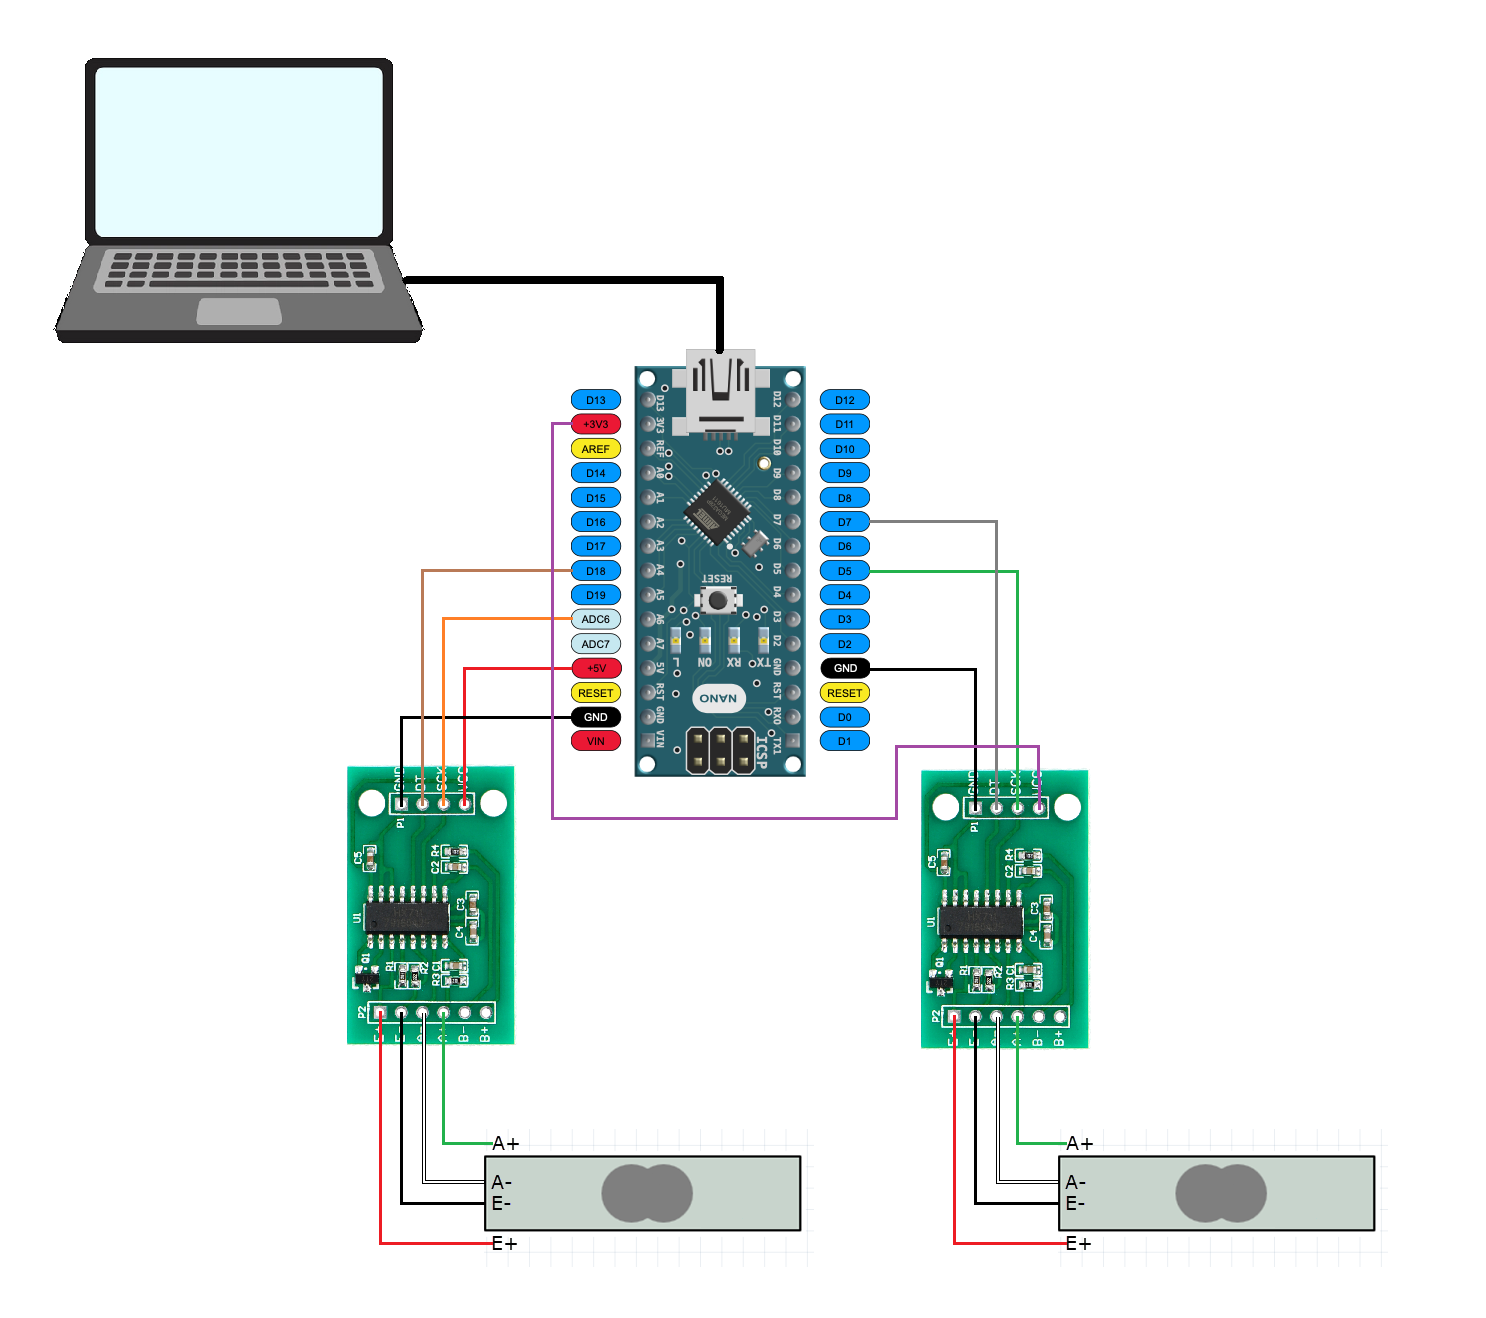
\includegraphics[width=0.8\textwidth]{img/Schaltungs-Aufbau.png}
    \caption{Gesamtaufbau Wägezelle mit Arduino Nano}
    \label{Gesamtaufbau-waegezelle-mit-Arduino-Nano}
\end{figure}
\\
Is die Hardware nun korrekt konfiguriert, muss die Software geschrieben werden die alles steuert.
In der Arduino IDE können mithilfe der passenden Library und einem selber geschriebenen Programm die Daten ausgelesen und gespeichert werden.
Der auf dem Arduino ausgeführte C-Code liest periodisch den analogen Wert des HX711 aus.
Zunächst muss der Sensor initialisiert werden.
Dies geschieht durch:
\begin{enumerate}
    \item \textbf{Angabe eines Kalibrationswertes}: Dieser Wert dient der genauen Gewichtsmessung.
    \item \textbf{Tara-Einstellung}: Die Waage wird auf 0 kg gesetzt, um sicherzustellen, dass nachfolgende Messungen korrekt sind.
\end{enumerate}
Nach der Initialisierung ist die Waage bereit, Messdaten auszugeben.
\\
Für die Ausgabe eines Messwerts werden die gemessenen Daten über den Serial-Port übertragen.
Dabei wird angegeben, ob die Messung von der linken oder rechten Waage stammt.
Die Ausgabe erfolgt beispielsweise wie folgt:
\begin{center}
    \begin{tabular}{l r}
        \texttt{Gewicht rechts [kg]:} & \texttt{-0.00118} \\
        \texttt{Gewicht links [kg]:}  & \texttt{-0.00321} \\
        \texttt{Gewicht rechts [kg]:} & \texttt{-0.00118} \\
        \texttt{Gewicht links [kg]:}  & \texttt{-0.00223} \\
    \end{tabular}
\end{center}
Der serielle Monitor verarbeitet die Ausgabe des Arduinos und ergänzt jeden Messwert mit einem Zeitstempel, der den Zeitpunkt angibt, zu dem der Messwert den Computer erreicht.
Dadurch wird es möglich, die seriellen Daten in Echtzeit als Graph über die Zeit darzustellen, wie in \autoref{fig:serial_output_example} veranschaulicht.
% %todo:
\begin{figure}[h!]
    \centering
    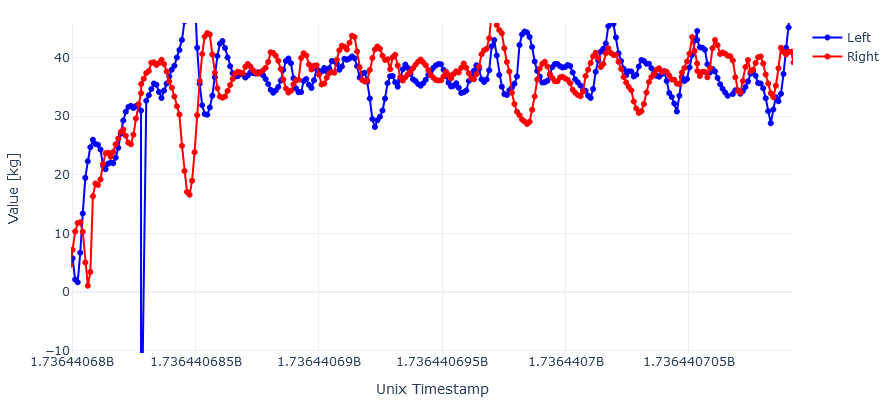
\includegraphics[width=0.7\textwidth]{img/serial_output_example.png} % Screenshot oder Beispiel
    \caption{Ausgabe der Messdaten mit Python}
    \label{fig:serial_output_example}
\end{figure}
\\
Alle Daten werden anschließend in einem CSV-Format gespeichert.
Sie können nun beliebig aufbereitet und analysiert werden.
% Der C Code auf dem Arduino liest periodisch den analogen Wert des HX711 aus, muss dafür aber zuerst initialisiert werden.
% Dazu wird ein Kalibrationswert angegeben und anschließend die Waage auf 0 kg getared.
% Nun ist die Waage initialisiert und bereit, Messdaten auszugeben.
% Soll ein Messwert ausgegeben werden, so werden die Daten an den Serial-Port ausgegeben, mit dem Hinweis, ob der Messwert von links oder rechts stammt.
% An dem Serial-Port angekommen werden die Daten von einem zweiten parallel laufenden Python Skript ausgewertet.
% Dabei können die Daten in Echtzeit in einer web App dargestellt werden und werden gleichzeitig aufgezeichnet im CSV-Format.
Diese Daten können nun auf verschiedene Art und Weisen mithilfe von Python dargestellt werden.\\
\\
\subsection{EMG Messung}
Im Rahmen des Messversuchsaufbaus, dargestellt in \autoref{fig:EMG-Messaufbau} wurde zunächst sichergestellt, dass die Probanden eine reproduzierbare Ausgangsposition für die Kniebeuge einnehmen konnten.
Hierzu wurden die Fußumrisse jedes Probanden auf einem großen Papier aufgezeichnet.
Dies diente als Orientierungshilfe, um die Standposition für die zweite Messung exakt wiederherstellen zu können.
\begin{figure}[h!]
    \centering
    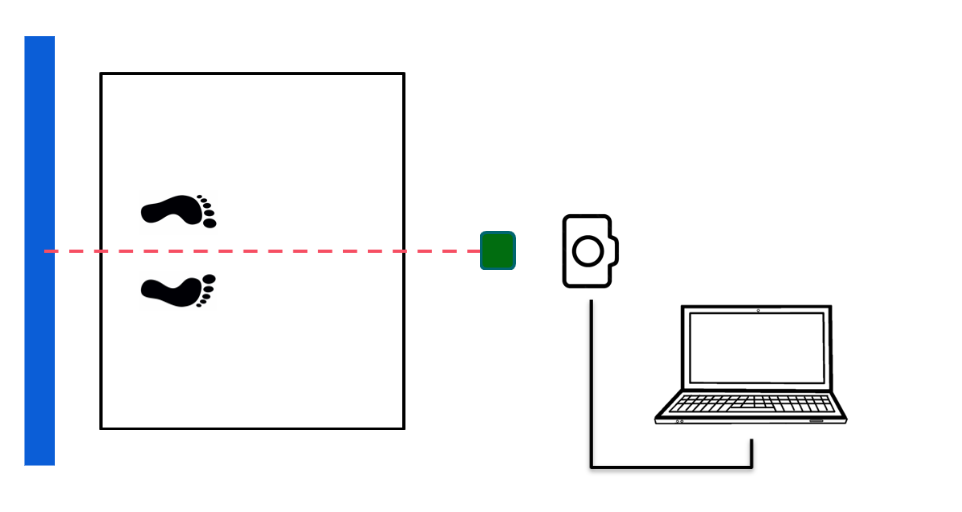
\includegraphics[width=0.8\linewidth]{img/Aufbau-EMG.png}
    \caption{EMG Messaufbau}
    \label{fig:EMG-Messaufbau}
\end{figure}
Zur korrekten Ausrichtung während der Bewegung wurde ein Baulaser in einer Entfernung von 1,5 Metern vor dem Probanden positioniert.
Dieser projizierte eine vertikale Linie, an der sich die Probanden vor jeder Messung neu ausrichten konnten.
Hinter dem Baulaser wurde eine Kamera installiert, die synchron mit einem PC und dem EMG-Messsystem (Elektromyografie) verbunden war.
\\
Für eine konsistente Bild- und Datenaufnahme wurde im Hintergrund ein Zeichenboard als gleichfarbige Kulisse positioniert.
Dies minimierte störende visuelle Einflüsse und erleichterte die anschließende Auswertung der aufgenommenen Daten.
Die EMG-Elektroden wurden gezielt am Quadrizeps platziert, um die Muskelaktivität differenziert zu messen.
Dabei wurden drei spezifische Positionen am Oberschenkel berücksichtigt:
innen am Vastus medialis, mittig am Rectus femoris und außen am Vastus lateralis.
An jedem Bein wurden jeweils eine Elektrode am rechten und linken Oberschenkel angebracht, um eine beidseitige Erfassung der Muskelaktivität während der Kniebeuge sicherzustellen.
 % !!!

\section{Ausgleichsübungen}
\input{txt/Ausgleichsübungen}

\section{Auswertung}
\subsection{Auswertung Wägezellen}
\subsubsection{Quantisierung der Gewichtsverteilung}
% Kalibrierung der Wägezelle?
Die von der Wägezelle übertragenen Gewichtsdaten der linken und rechten Seite sollen beschreiben wie sehr die jeweilige Seite belastet wird.
Da die EMG Messungen nicht gleichzeitig mit den Wägezellen Messungen durchgeführt wurden, können die Daten nicht direkt miteinander verglichen werden.
Um dennoch Erkenntnisse aus den Wägezellen Daten zu gewinnen, sind folgende Überlegungen angestellt worden:
\begin{itemize}
  \item Die Phase in der die Person auf die Waage tritt und in der sie wieder absteigt wird für die Auswertung nicht berücksichtigt.
  In \autoref{fig: Differenz - Any} sind diese Phasen an den negativen und positiven Peaks am Anfang und am Ende des Graphen zu erkennen.
  \item Ein über die Zeit verteilt deutliche höheres Gewicht auf einer Seite entspricht einer stärkeren Belastung dieser Seite.
  \item Mathematische Aufbereitung der Rohdaten:
    \item[$\cdot$] $m_{links} - m_{rechts} =$ Differenz zwischen Masse links und Masse rechts über die Zeit, zeigt Momentanwerte (dargestellt ist \autoref{fig: Differenz - Any})
    \item[$\cdot$] Integral über \autoref{fig: Differenz - Any} ist der kumulative Unterschied der Gewichtsbelastung zwischen links und rechts, zeigt Langzeit-Asymmetrie (dargestellt in \autoref{fig:weight_distribution_integral_any})
    \item[$\cdot$] positiver Wert des Integrals $\rightarrow$ höhere Belastung der linken Seite
    \item[$\cdot$] negativer Wert des Integrals $\rightarrow$ höhere Belastung der rechten Seite
\end{itemize}

\begin{figure}
  \centering
  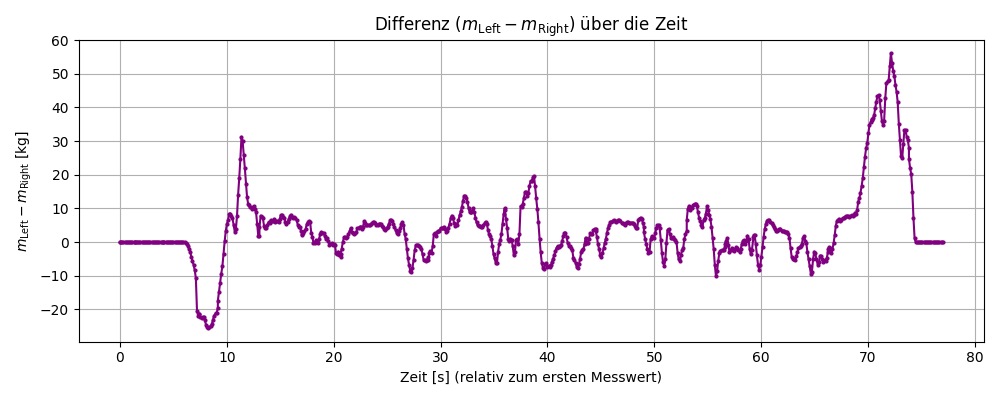
\includegraphics[width=0.7\linewidth]{img/pyplots/Differenz - Any.png}\\
  \caption{Differenz der Gewichtsverteilung von Any}
  \label{fig: Differenz - Any}
\end{figure}

% \begin{align}
%   \int \Delta m(t) ~dt &\approx \sum_{i=1}^{n} \Delta m_i \cdot \Delta t_i
%   \label{eq:integral_differenz} \\
%   %
% \end{align}

\begin{figure}
  \centering
  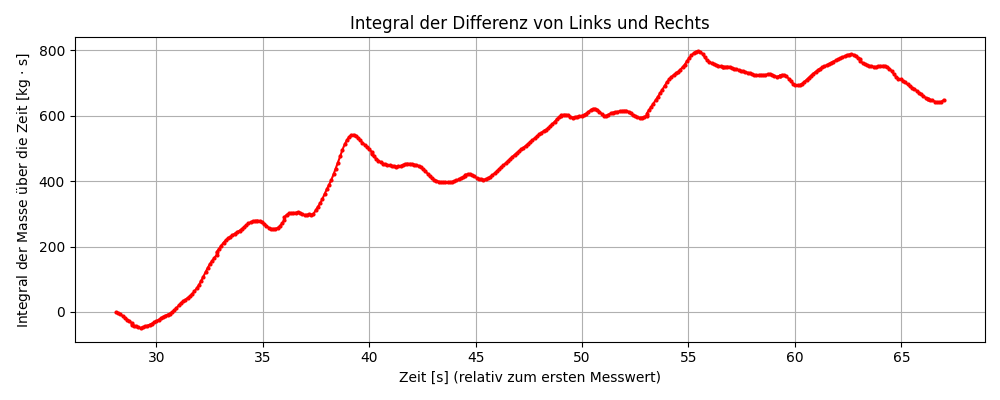
\includegraphics[width=0.7\linewidth]{img/pyplots/Integral der Differenz - Any.png}\\
  \caption{Integral der Differenz der Gewichtsverteilung von Any}
  \label{fig:weight_distribution_integral_any}
\end{figure}
Der in \autoref{fig:weight_distribution_integral_any} dargestellte Graph zeigt einen kontinuierlichen Anstieg, was einer stärkeren Belastung der linken Seite über den betrachteten Zeitraum entspricht. \\
\\
Der in \autoref{fig:weight_distribution_integral_giorgio} dargestellte Verlauf liegt zum großen Teil unterhalb der Nulllinie, was bedeutet, dass die rechte Seite kumulativ mehr Gewicht getragen hat als die linke.
Zwischen 30 und 40 Sekunden steigt der Graph einmal deutlich an und fällt ab ca. Sekunde 37 wieder ab, was auf einen Ausgleichsversuch hindeuten könnte. Die Gewichtsverteilung bleibt aber rechtslastig.
\begin{figure}
  \centering
  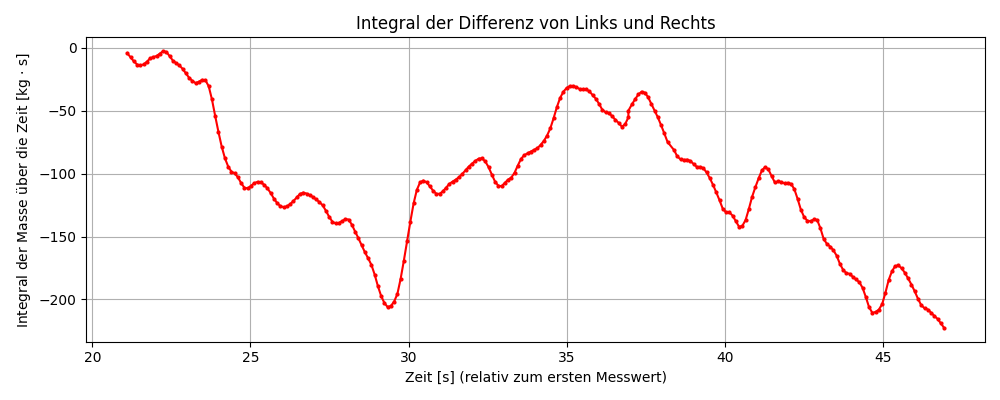
\includegraphics[width=0.7\linewidth]{img/pyplots/Integral der Differenz - Giorgio.png}\\
  \caption{Integral der Differenz der Gewichtsverteilung von Giorgio}
  \label{fig:weight_distribution_integral_giorgio}
\end{figure}
Auch der in \autoref{fig:weight_distribution_integral_max} dargestellte Graph zeigt eine negtaive Tendenz und somit eine starke rechtsseitige Belastung. Der wellenartige Verlauf könnten Korrekturversuch sein, trotzdem wird die rechtsseitige Belastung stetig größer.
\begin{figure}
  \centering
  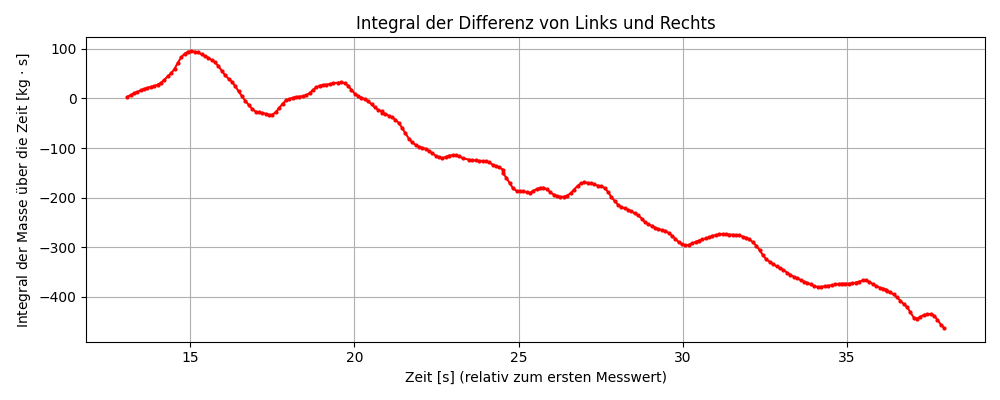
\includegraphics[width=0.7\linewidth]{img/pyplots/Integral der Differenz - Max.png}\\
  \caption{Integral der Differenz der Gewichtsverteilung von Max}
  \label{fig:weight_distribution_integral_max}
\end{figure}
\\
Einen sehr auffälligen Verlauf zeigt der letzte Graph \autoref{fig:weight_distribution_integral_felix}.
Das Integral steigt kontinuierlich über den gesamten Zeitraum.
Es gibt kaum wellenartige Schwankungen, was darauf hinweist das die linke Seite durchgehend stärker belastet wird als die rechte und scheinbar keine Korrekturversuche stattfanden.
Die Gewichtsverlagerung ist zwar stabil, aber sehr einseitig.
\begin{figure}
  \centering
  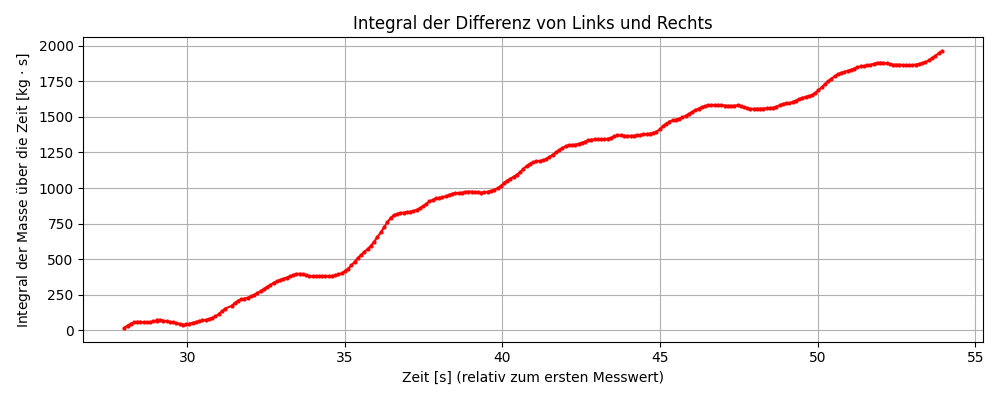
\includegraphics[width=0.7\linewidth]{img/pyplots/Integral der Differenz - Felix.png}\\
  \caption{Integral der Differenz der Gewichtsverteilung von Felix}
  \label{fig:weight_distribution_integral_felix}
\end{figure}
\\
\\
Was auffällt ist, dass in den Rohdaten die sechs einzelnen Kniebeugen nicht voneinander unterscheidbar sind.
Für zukünftige Messungen wäre es daher zu empfehlen, pro Kniebeuge nur einen Graphen zu erstellen, so dass die Fehlbelastungen besser mit dem einzelnen Bewegungsablauf in Einklang gebracht werden können.\\
\\
Trotzdem hat die Auswertung und mathematische Aufbereitung der Daten der Wägezellen sinnvolle Ergebnisse erbracht. Und kann für auch für zukünftige Auswertungen angepasst werden.
\subsection{Auswertung EMG}
\subsubsection{Symmetrie-Index (SI): Bedeutung und Berechnung}

Der Symmetrie-Index (SI) ist eine Maßzahl, die den Grad der Asymmetrie zwischen zwei Körperseiten - beispielsweise der linken und rechten Seite eines Muskels - beschreibt.
Er wird häufig in der Biomechanik, Physiotherapie und Sportwissenschaft verwendet, um muskuläre Dysbalancen zu bewerten.
Die Berechnung erfolgt mit folgender Formel: \cite{bmcsportsscimedrehabil}

\begin{equation}
    SI = \frac{|X_1 - X_2|}{\frac{X_1 + X_2}{2}} \cdot 100
\end{equation}
Wobei $X_1$ und $X_2$ die Mittelwerte der Muskelaktivität auf der linken ($X_1$) und rechten ($X_2$) Seite sind.
\\
Interpretation des Symmetrie-Index:
Ein höherer SI-Wert weist auf eine stärkere Asymmetrie zwischen den beiden Seiten hin.
Ein niedrigerer SI-Wert deutet auf eine gleichmäßigere Belastung und damit auf eine bessere Symmetrie hin.

\subsubsection{Symmetrie-Index vor und nach den Ausgleichsübungen}

Die durchschnittlichen Symmetrie-Index-Werte der drei analysierten Muskeln (Rectus femoris, Vastus lateralis, Vastus medialis) wurden vor und nach den Ausgleichsübungen berechnet. Zudem wurde ermittelt, wie viele Probanden eine Verbesserung des Symmetrie-Indexes (SI) zeigten:

\begin{table}[htbp]
  \centering
    \begin{tabular}{|c|c|c|c|}
    \hline
    \textbf{Muskel} & \textbf{Durchschnitt SI vor \%} & \textbf{Durchschnitt SI nach \%} & {\textbf{Verbesserungen [\%]}} \\
    \hline
    Rectus femoris & \multicolumn{1}{c|}{18.06} & 13.18 & 75 \\
    \hline
    Vastus lateralis & 24.24 & 18.70 & 75 \\
    \hline
    Vastus medialis & 17.84 & 15.05 & 75 \\
    \hline
    \end{tabular}%
    \caption{durchschnittliche SI-Werte}
  \label{tab:durchschnittliche-SI-Werte}%
\end{table}%

\subsubsection{Interpretation der Ergebnisse}
\begin{itemize}
    \item Rectus femoris (innen)
    Der durchschnittliche Symmetrie-Index hat sich von 18.06 $\%$ auf 13.18 $\%$ verbessert.
    Bei allen drei Probanden wurde eine Verbesserung festgestellt.
    \textbf{Interpretation:} Die Ausgleichsübungen waren für diesen Muskel besonders effektiv, da die Symmetrie deutlich zugenommen hat.
    \item Vastus lateralis (außen)
    Der Symmetrie-Index hat sich von 24.24 $\%$ auf 18.70 $\%$ verbessert.
    Auch hier zeigten alle drei Probanden Verbesserungen.
    \textbf{Interpretation:} Der Vastus lateralis war vor den Übungen der asymmetrischste Muskel, aber die Übungen haben die Symmetrie erfolgreich gesteigert.
    \item Vastus medialis (innen)
    Der Symmetrie-Index hat sich von 17.84 $\%$ auf 15.05 $\%$ verbessert.
    Bei allen drei Probanden wurde eine Verbesserung festgestellt.
    \textbf{Interpretation:} Die Verbesserungen sind weniger ausgeprägt im Vergleich zu den anderen Muskeln, was darauf hinweist, dass der Muskel bereits eine bessere Ausgangssymmetrie hatte.
\end{itemize}

\subsubsection{Ergebnisse der EMG Messungen}
\begin{itemize}
    \item Die Ausgleichsübungen führten bei 3 von 4 Probanden zu einer Verbesserung der Symmetrie.
    \item Besonders der Rectus femoris und der Vastus lateralis profitierten von den Übungen, da bei ihnen die Asymmetrien am stärksten reduziert wurden.
    \item Der Vastus medialis hatte bereits vor den Übungen eine relativ gute Symmetrie, weshalb die Verbesserungen hier weniger ausgeprägt ausfielen.
\end{itemize}

\subsection{Mögliche Gründe für fehlende Verbesserungen des Symmetrie-Indexes}

Auch wenn bei diesem Datensatz durchgängig Verbesserungen festgestellt wurden, könnten in anderen Fällen folgende Faktoren dafür sorgen, dass keine Verbesserung des Symmetrie-Indexes erzielt wird:

\begin{itemize}
    \item 1. Unzureichende Wirksamkeit der Übungen:\\
    Die Übungen könnten nicht spezifisch genug gewesen sein, um die Asymmetrie in den betroffenen Muskeln auszugleichen.\\
    Eine ungleichmäßige Belastung während der Übungen könnte die Symmetrie sogar verschlechtern.\\
    %
    \item 2. Individuelle Unterschiede: \\
    Unterschiede im Fitnesslevel, in der Anatomie oder in der Bewegungskoordination der Probanden könnten den Effekt der Übungen verringern.\\
    Eine vorhandene Verletzung oder ein muskuläres Ungleichgewicht könnte die Symmetrie nicht vollständig ausgleichbar machen.\\
    %
    \item 3. Messfehler:\\
    Eine unpräzise Platzierung der EMG-Elektroden könnte zu falschen Werten führen, die den Effekt der Übungen verfälschen.\\
    Signalrauschen oder Störungen im EMG-System könnten die Datenqualität beeinträchtigen.\\
    %
    \item 4. Ermüdung oder Tageszeit-Effekte:\\
    Die Messungen vor und nach den Übungen könnten durch den Ermüdungszustand der Muskeln oder die Tageszeit beeinflusst worden sein.\\
    %
    \item 5. Lerneffekt:\\
    Die Verbesserungen könnten nicht auf die Übungen, sondern auf eine bessere Koordination der Probanden während der Messungen (Übungseffekt) zurückzuführen sein.
\end{itemize}


 % !!!

\section{Fazit}
Das Projekt zeigte, dass asymmetrische Belastungen bei Kniebeugen häufig vorkommen und sowohl durch Fehlhaltungen als auch durch muskuläre Dysbalancen bedingt sein können.
Die erste Messung zeigte bei allen Probanden eine ungleichmäßige Muskelbelastung, was eine erhöhte Belastung auf einer Seite zur Folge haben kann.
Nach dem regelmäßigen Training mit spezifischen Ausgleichsübungen konnte eine deutliche Verbesserung des Symmetrie-Indexes festgestellt werden.
Das verdeutlicht die Bedeutung von gezielten Korrekturübungen zur Prävention von Verletzungen und zur Optimierung von Bewegungsabläufen.
\\
\\
Obwohl nicht alle Dysbalancen komplett beseitigt werden konnten, zeigt das Projekt dennoch, dass gezielte Übungen einen spürbaren Einfluss auf die Symmetrie der Muskelbelastung haben.
Unterschiede in der Anatomie oder neurologische Faktoren könnten eine Rolle spielen, warum einige Asymmetrien bestehen bleiben.
Ein Verbesserungsvorschlag für zukünftige Versuche wäre, die Wägezellen sowohl vor als auch nach den Ausgleichsübungen einzusetzen, um eine vorher-nachher-Analyse anhand vergleichbarer Messdaten zu ermöglichen.
Die Reduktion der Asymmetrie konnte daher primär durch die EMG-Daten nachgewiesen werden.
Auch interessant wäre die Analyse einer einzelnen Kniebeuge mit den Wägezellen gewesen,  um die Bewegungsabläufe gezielter mit den Messwerten abzugleichen und asymmetrische Belastungen in spezifischen Phasen der Übung besser zu erkennen.
\\
\\
Für zukünftige Untersuchungen wäre es spannend, weitere Messungen durchzuführen, um den langfristigen Effekt der Übungen zu überprüfen und ob die Verbesserungen von dauer sind oder ab wann diese abklingen.
Auch interessant wäre die wöchentliche Verbesserung durch die Ausgleichsübungen zu analysieren, ob diese linear verläuft oder sich sprunghaft verbessert.
\\
Obwohl die Stichprobe mit nur vier Probanden sehr klein ist und die Ergebnisse daher nicht statistisch aussagekräftig sind, ist dennoch bemerkenswert, dass eine klare Verbesserung des Symmetrie-Indexes festgestellt werden konnte.
Dies zeigt, dass selbst mit kleinen Stichprobe interessante Einblicke gewonnen werden können.
\\
\\
Zusammenfassend zeigt das Projekt, dass asymmetrische Muskelbelastungen ein verbreitetes Phänomen sind, das durch gezielte Übungen reduziert werden kann. Dies hat sowohl für Freizeitsportler als auch für die physiotherapeutische Praxis Relevanz.

\clearpage
\addcontentsline{toc}{section}{Bibliography}
\printbibliography

\clearpage
\pagenumbering{roman}
\appendix

\addcontentsline{toc}{section}{Anhang}
\section*{Anhang}
% 





% Include all PDFs from the img directory
\subsection*{Any Außen - Vorher}
\includegraphics[width=.9\textwidth]{img/pdfs/Any_Außen_1.pdf}
\clearpage

\subsection*{Any Mitte - Vorher}
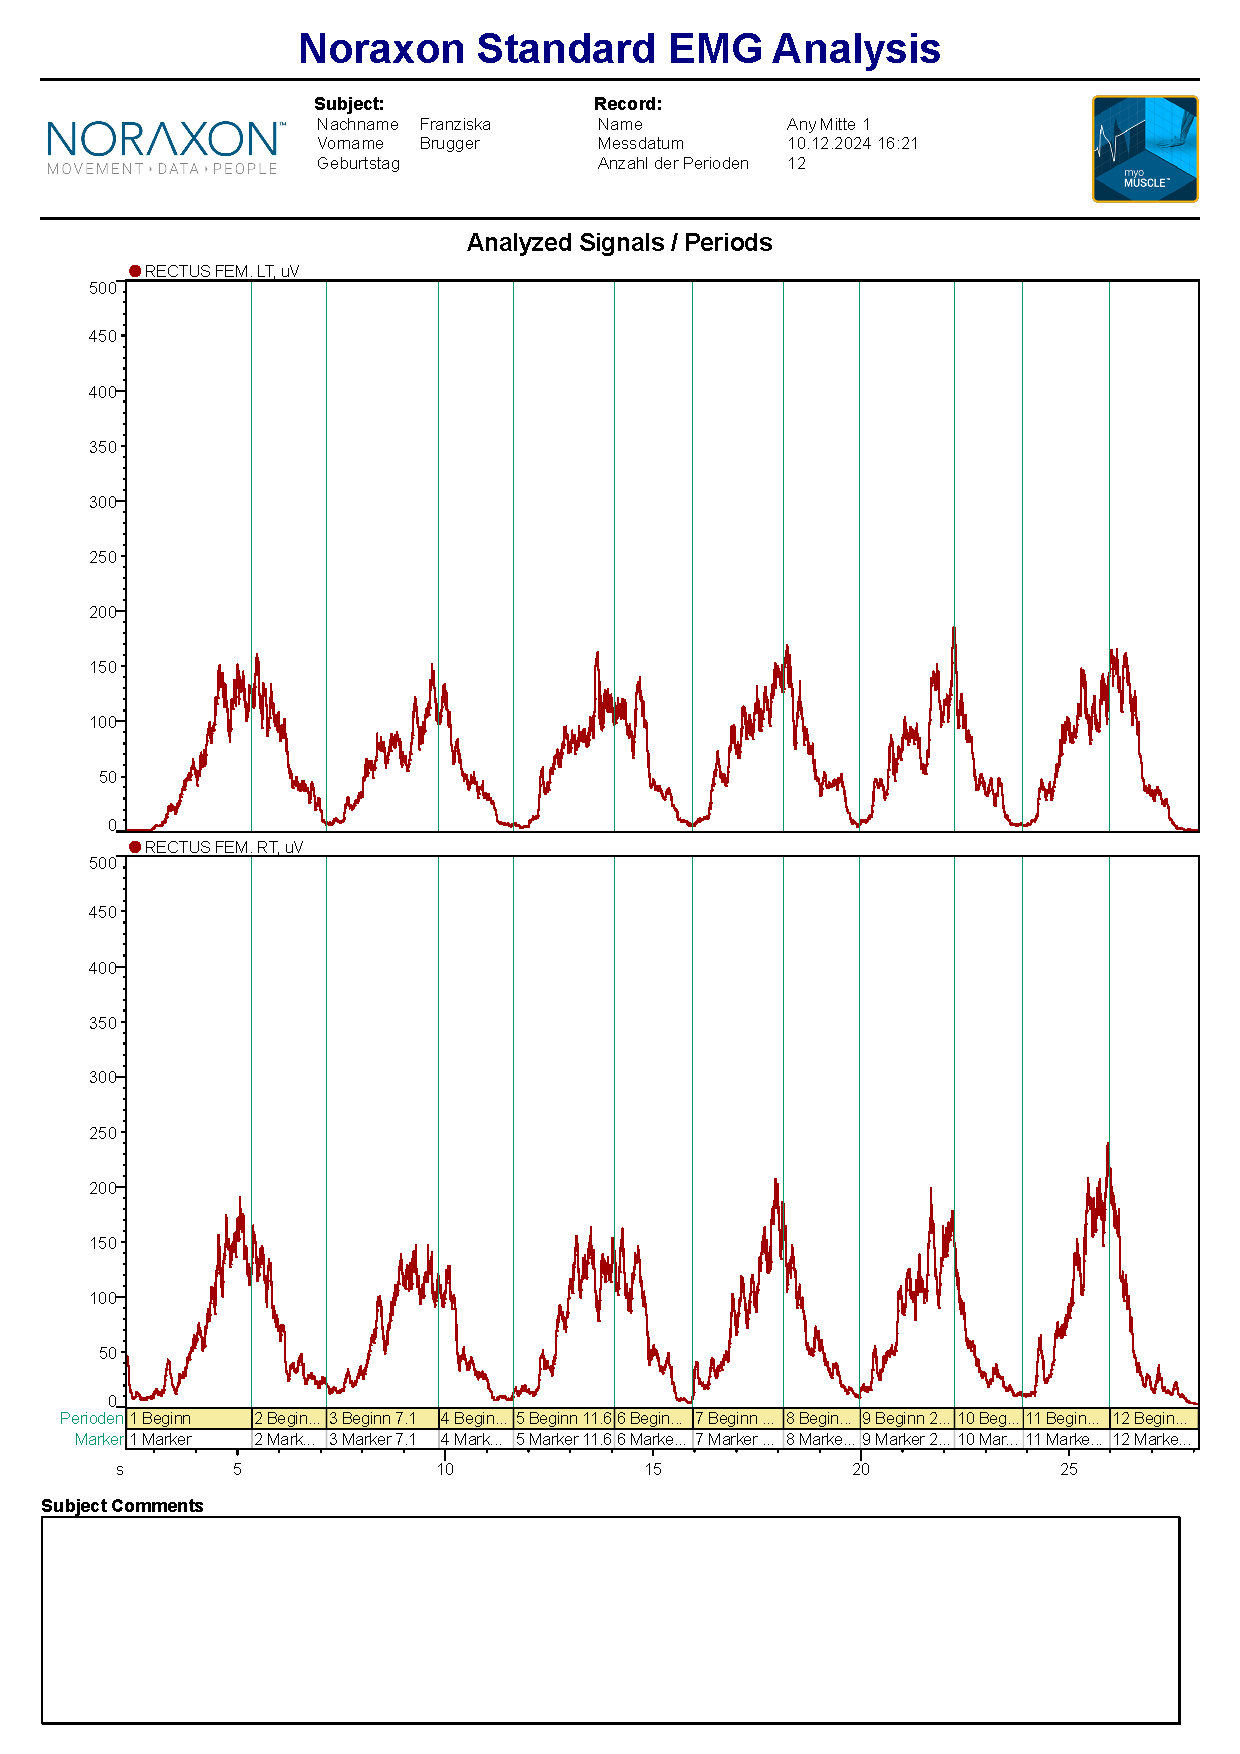
\includegraphics[width=.9\textwidth]{img/pdfs/Any_Mitte_1.pdf}
\clearpage

\subsection*{Any Innen - Vorher}
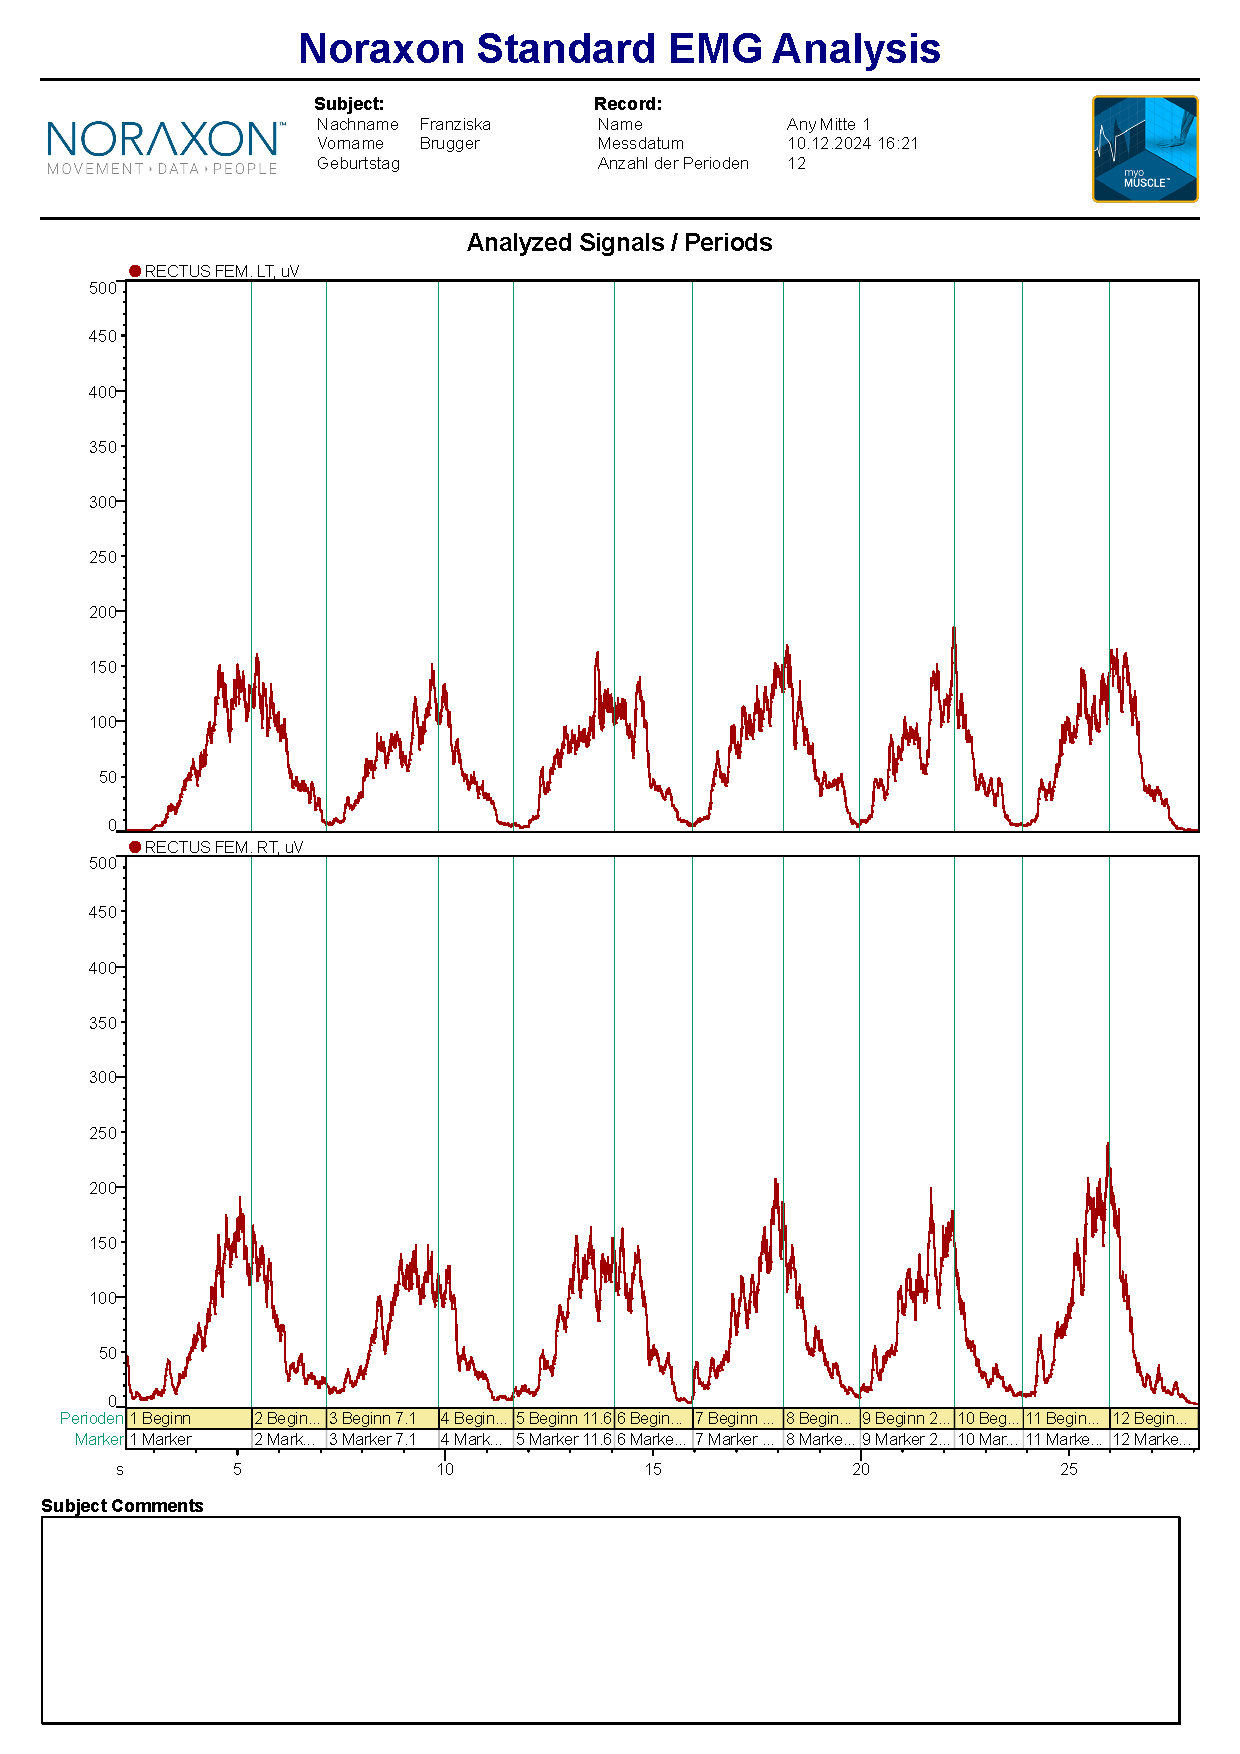
\includegraphics[width=.9\textwidth]{img/pdfs/Any_Mitte_1.pdf}
\clearpage

\subsection*{Any Außen - Nachher}
\includegraphics[width=.9\textwidth]{img/pdfs/Any_2_außen.pdf}
\clearpage

\subsection*{Any Mitte - Nachher}
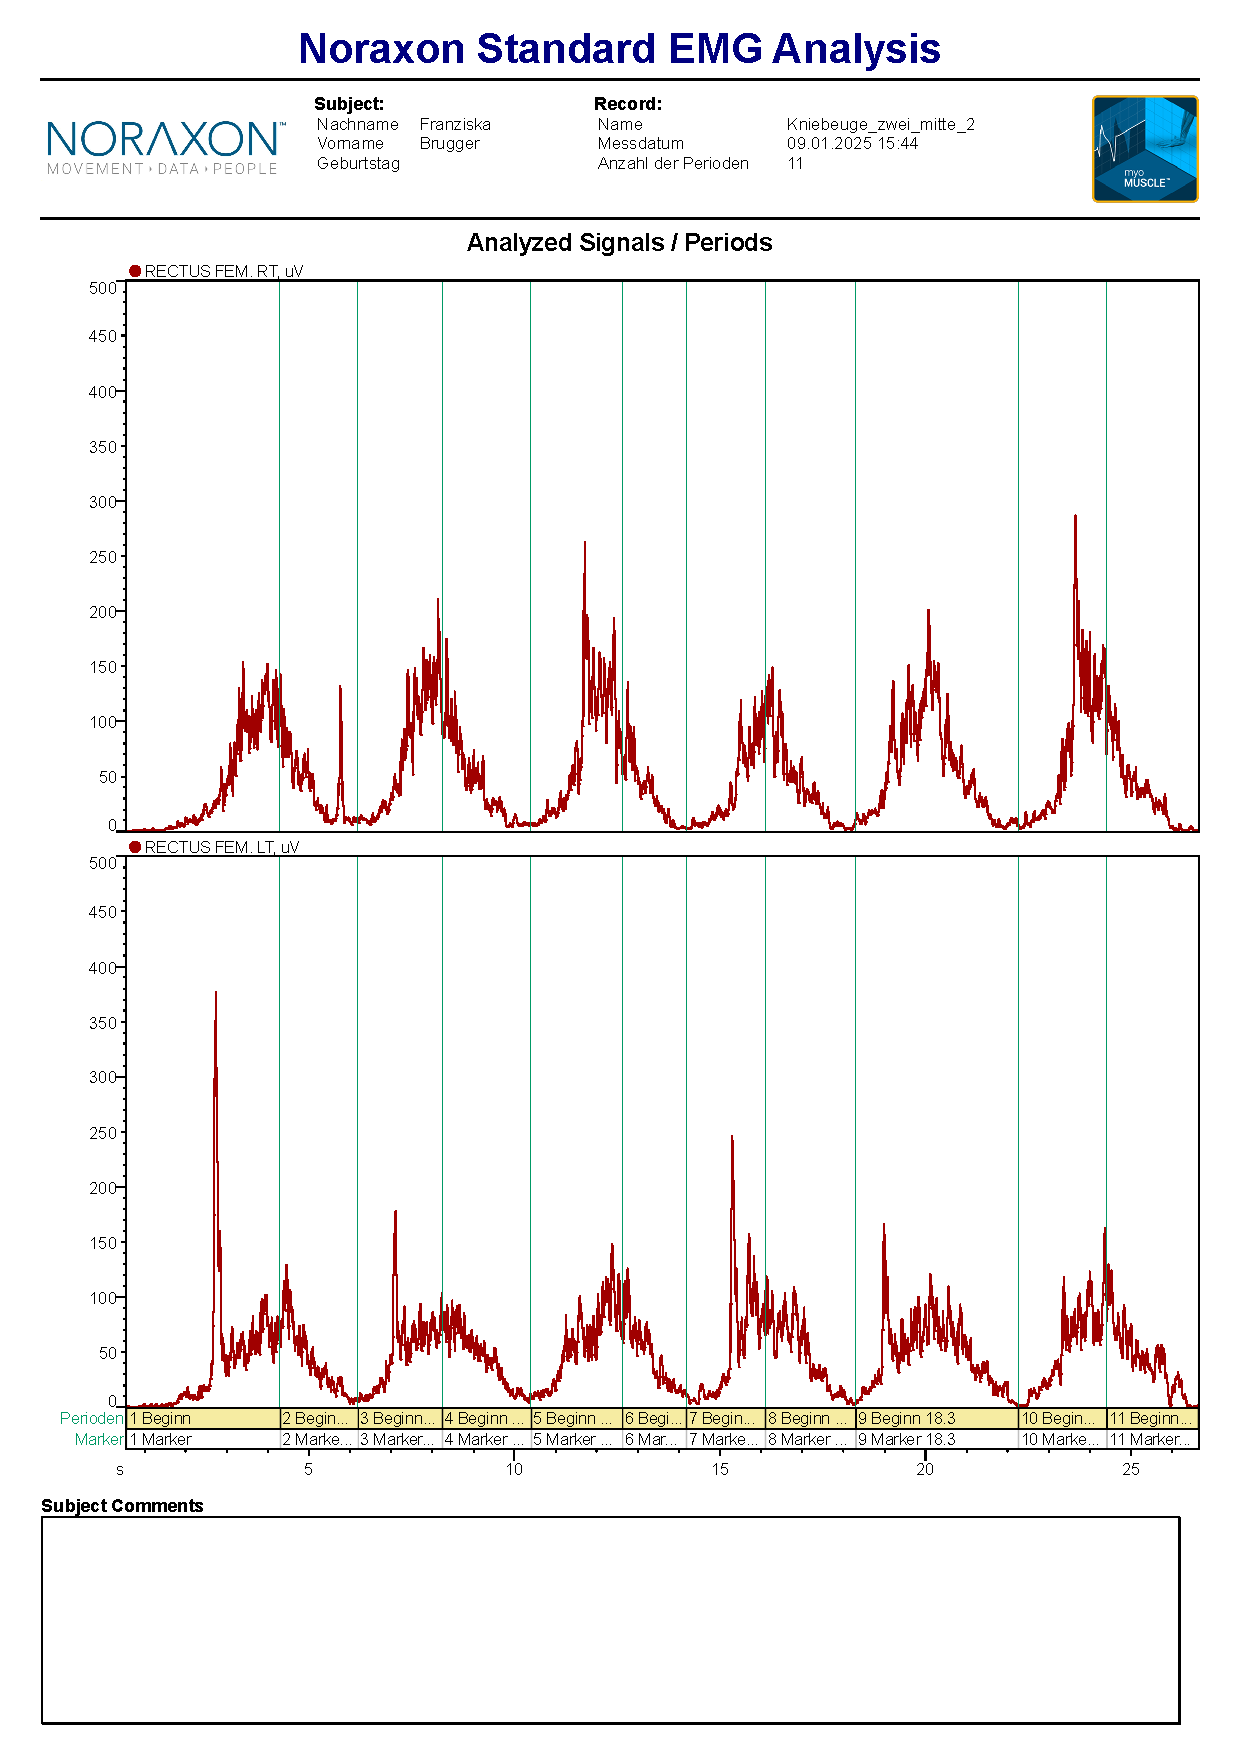
\includegraphics[width=.9\textwidth]{img/pdfs/Any_2_mitte.pdf}
\clearpage

\subsection*{Any Innen - Nachher}
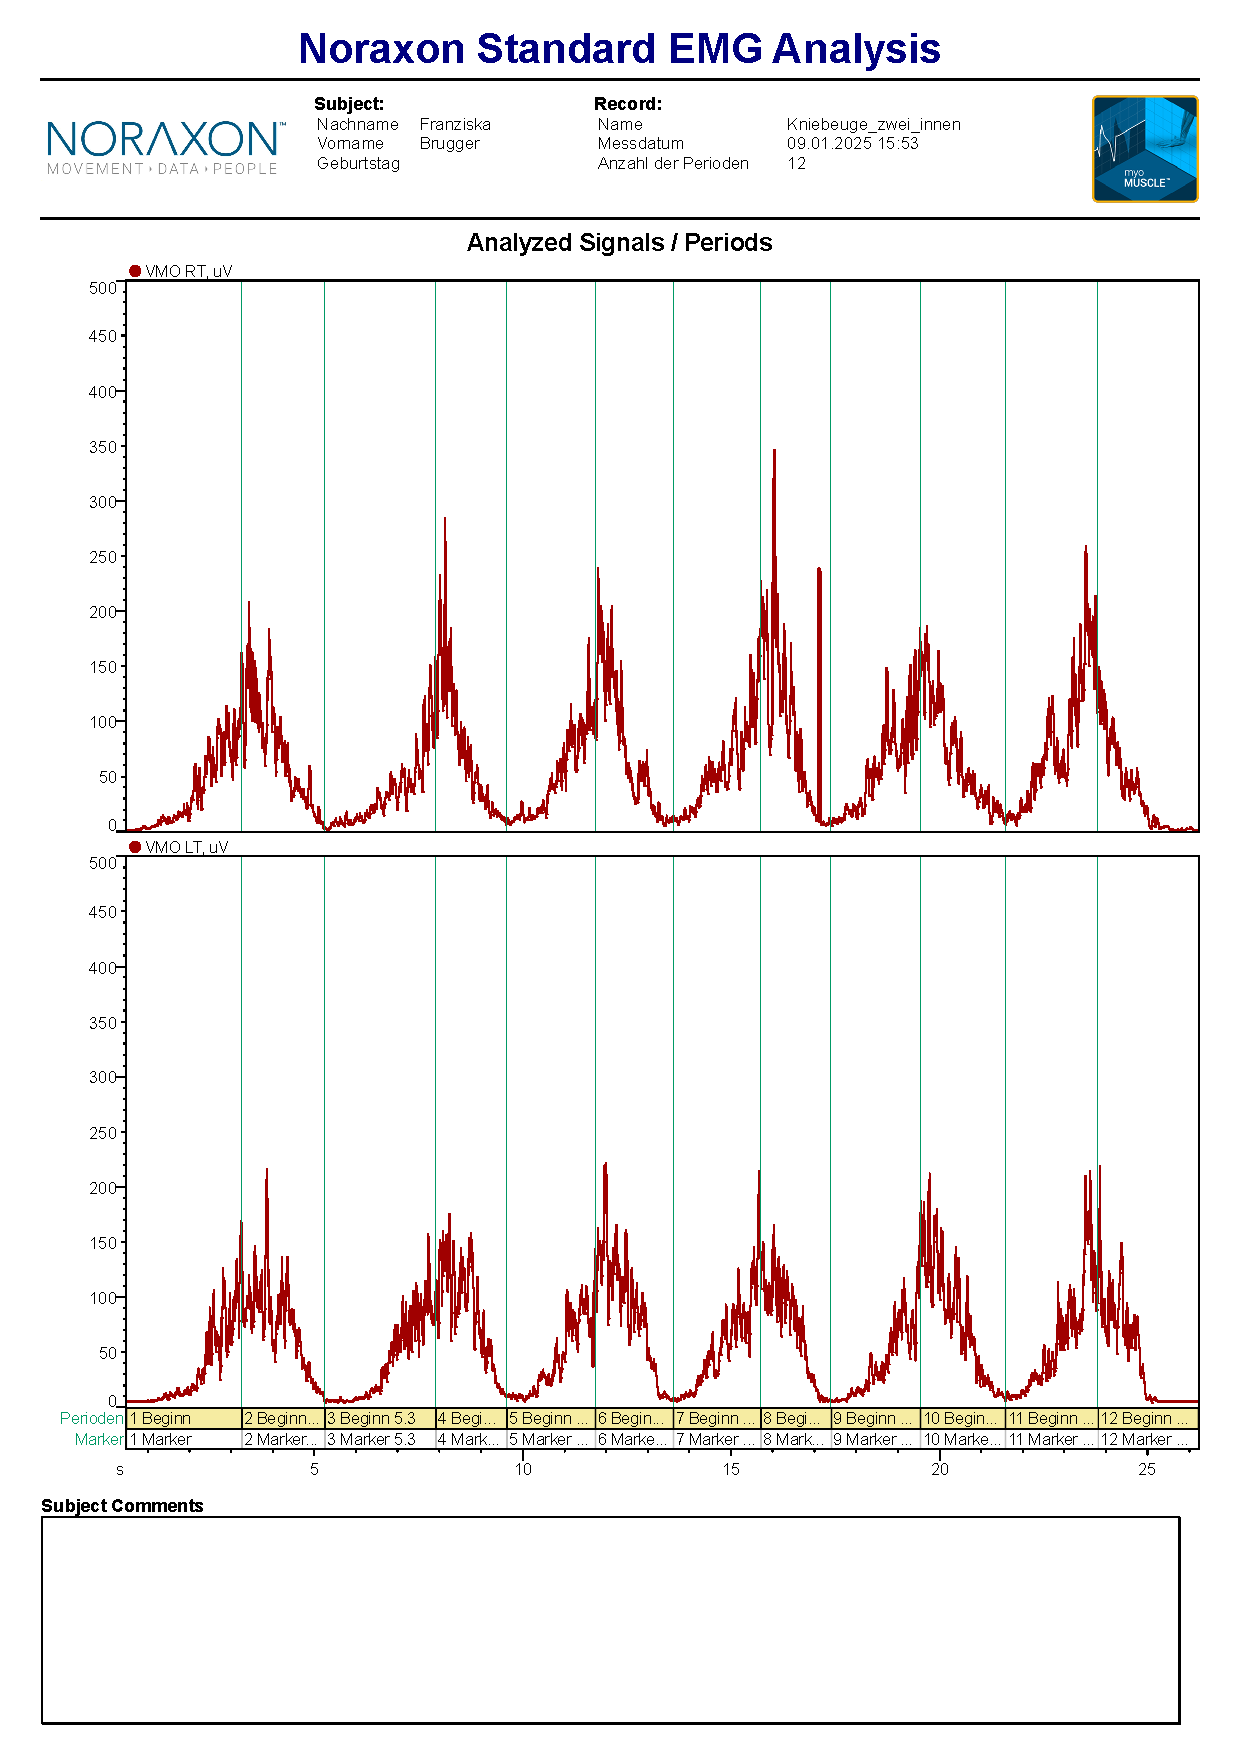
\includegraphics[width=.9\textwidth]{img/pdfs/Any_2_innen.pdf}
\clearpage

\subsection*{Felix Außen - Vorher}
\includegraphics[width=.9\textwidth]{img/pdfs/Felix_Außen_1.pdf}
\clearpage

\subsection*{Felix Mitte - Vorher}
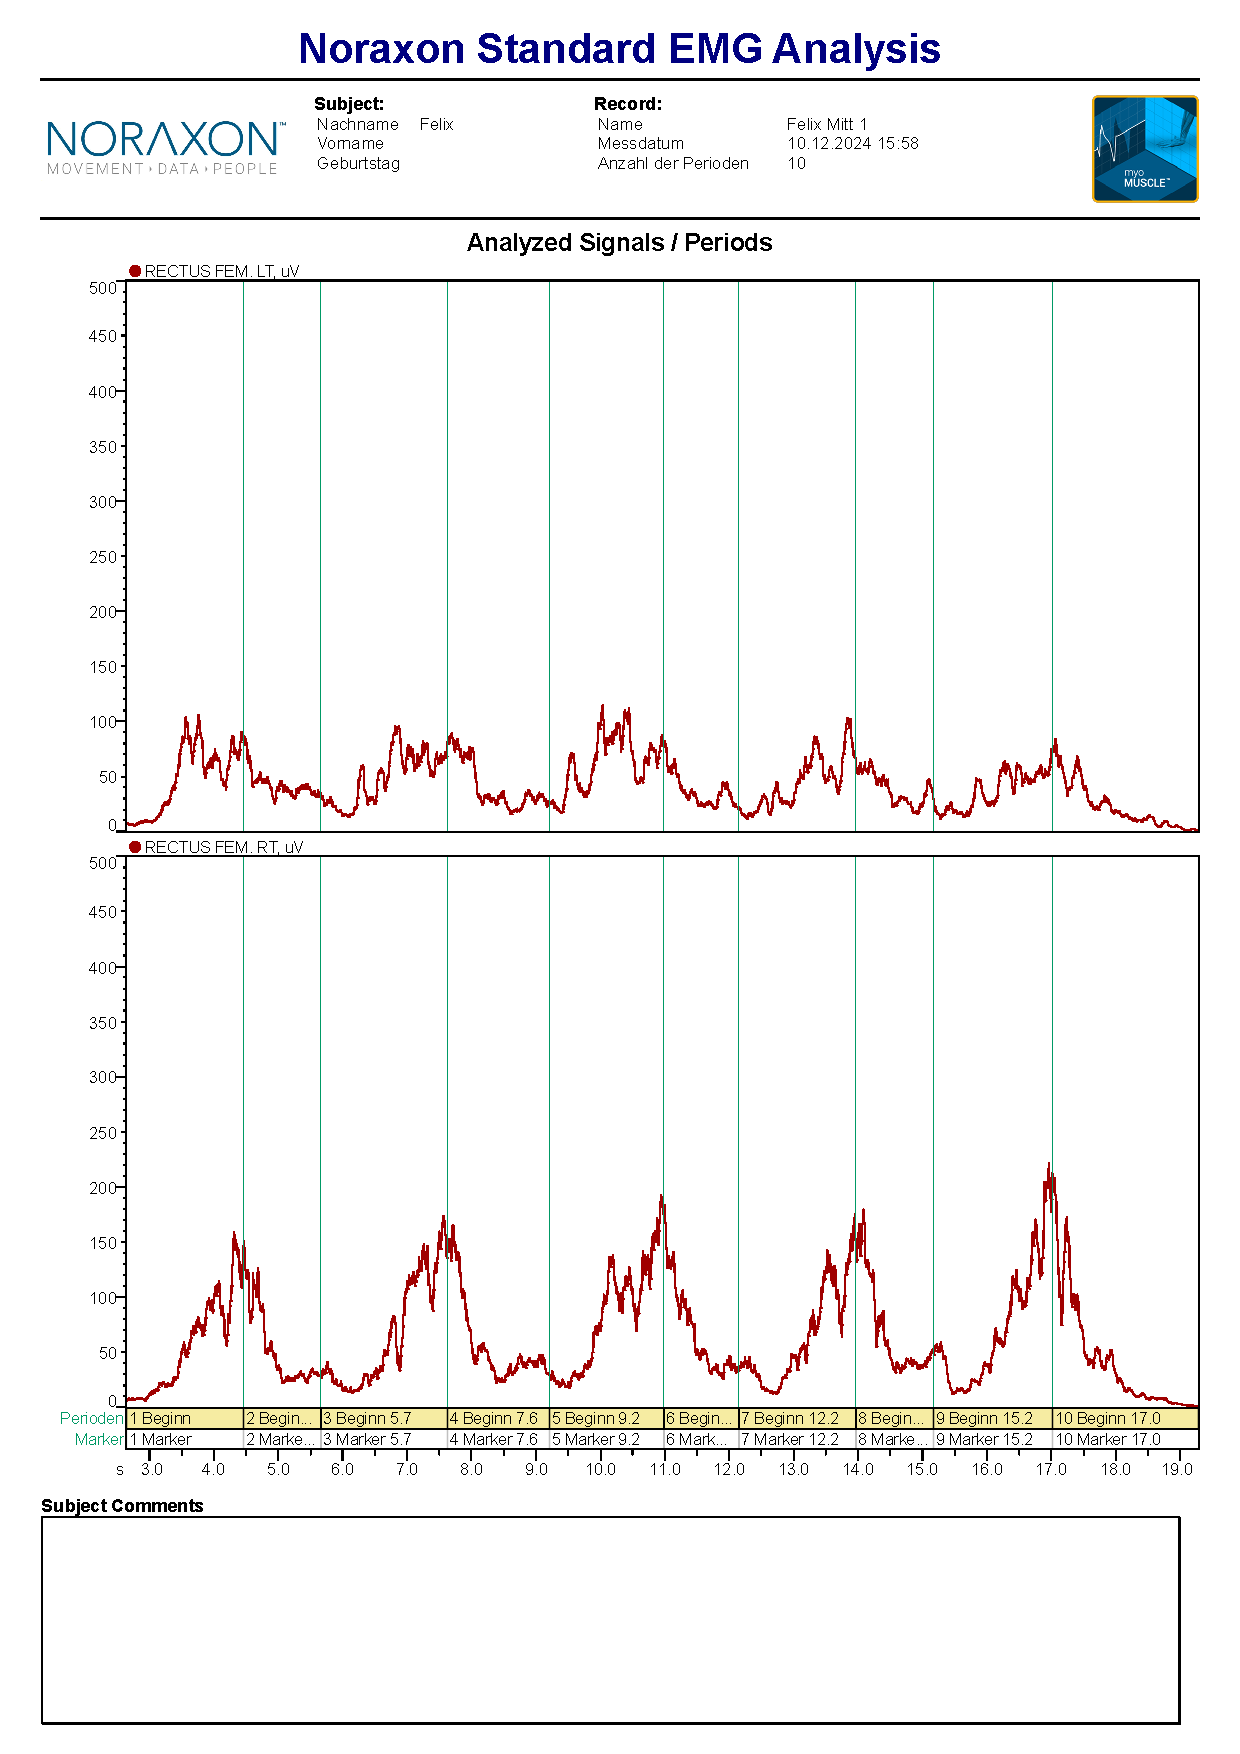
\includegraphics[width=.9\textwidth]{img/pdfs/Felix_Mitte_1.pdf}
\clearpage

\subsection*{Felix Innen - Vorher}
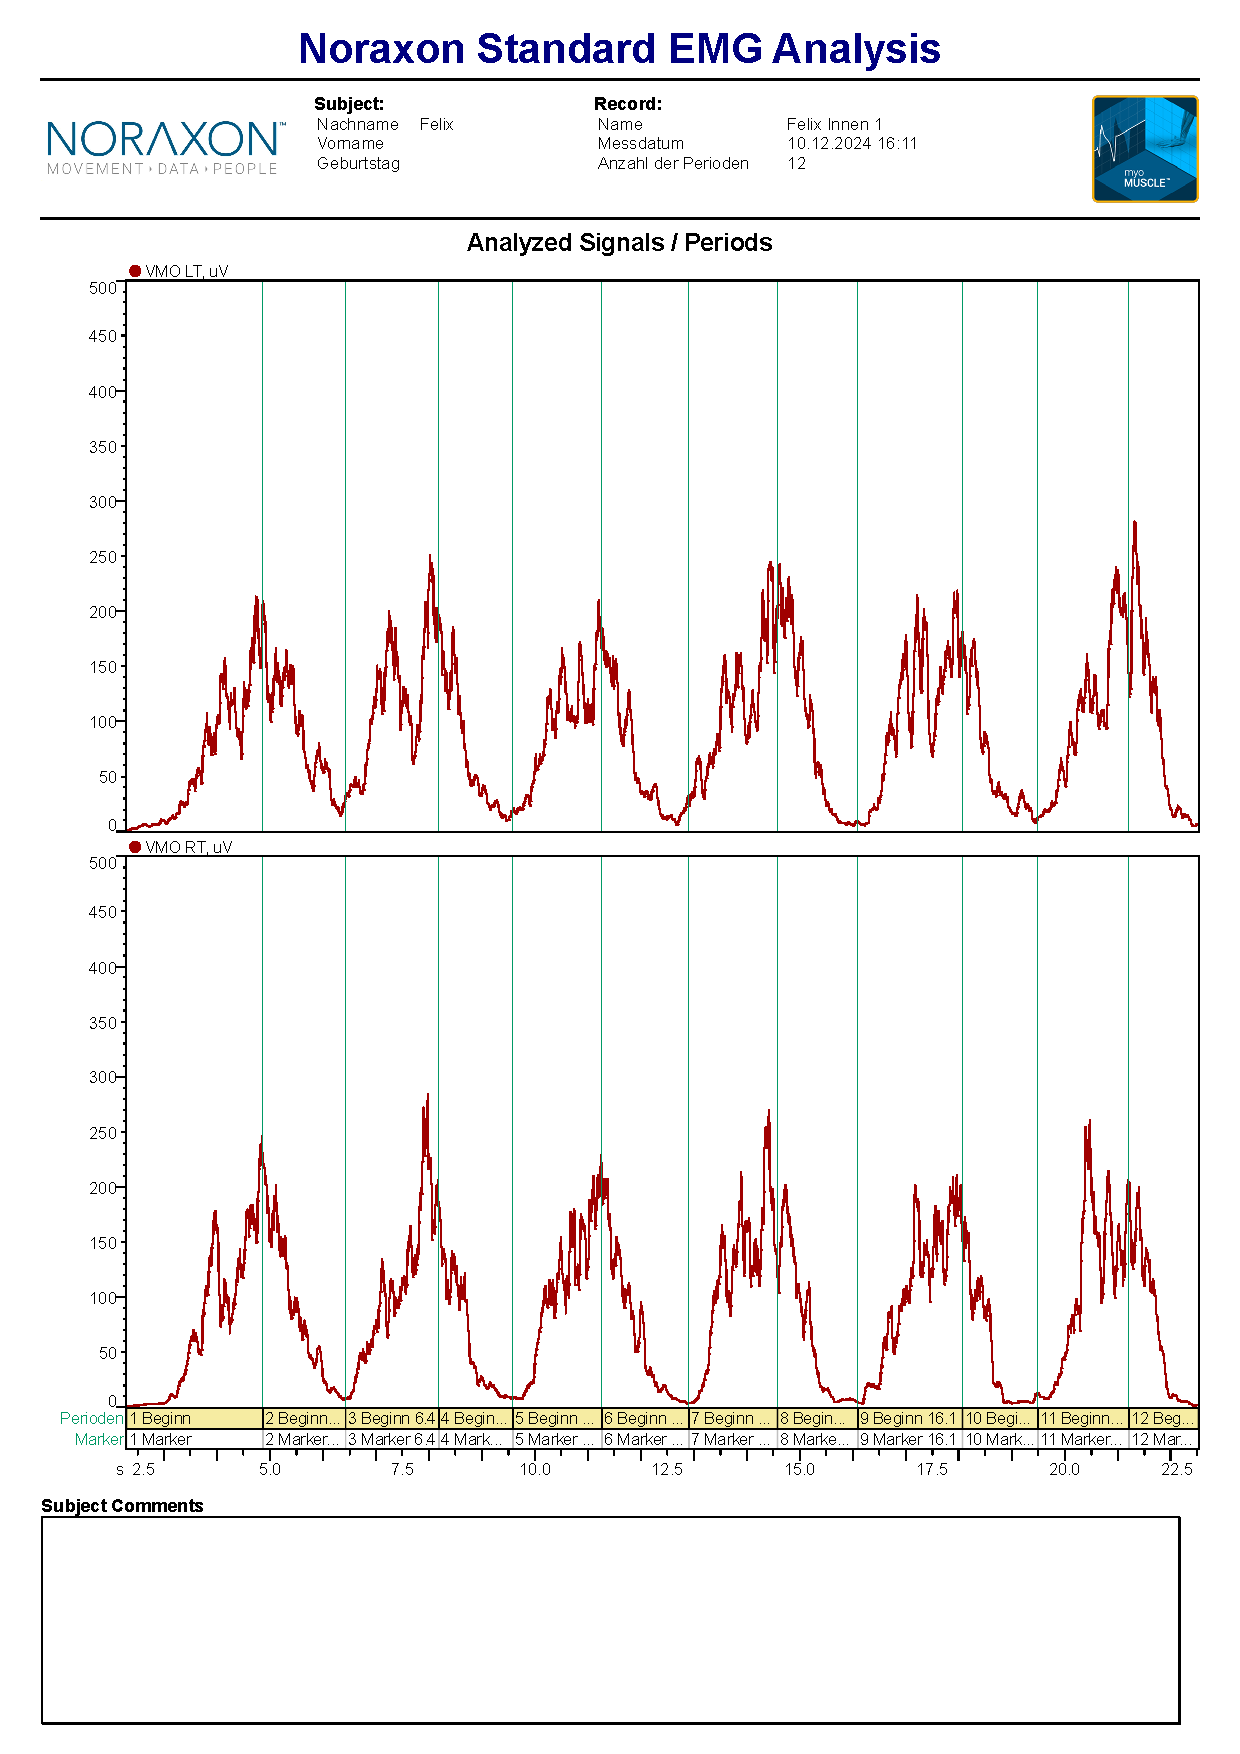
\includegraphics[width=.9\textwidth]{img/pdfs/Felix_Innen_1.pdf}
\clearpage

\subsection*{Felix Außen - Nachher}
\includegraphics[width=.9\textwidth]{img/pdfs/Felix_2_außen.pdf}
\clearpage

\subsection*{Felix Mitte - Nachher}
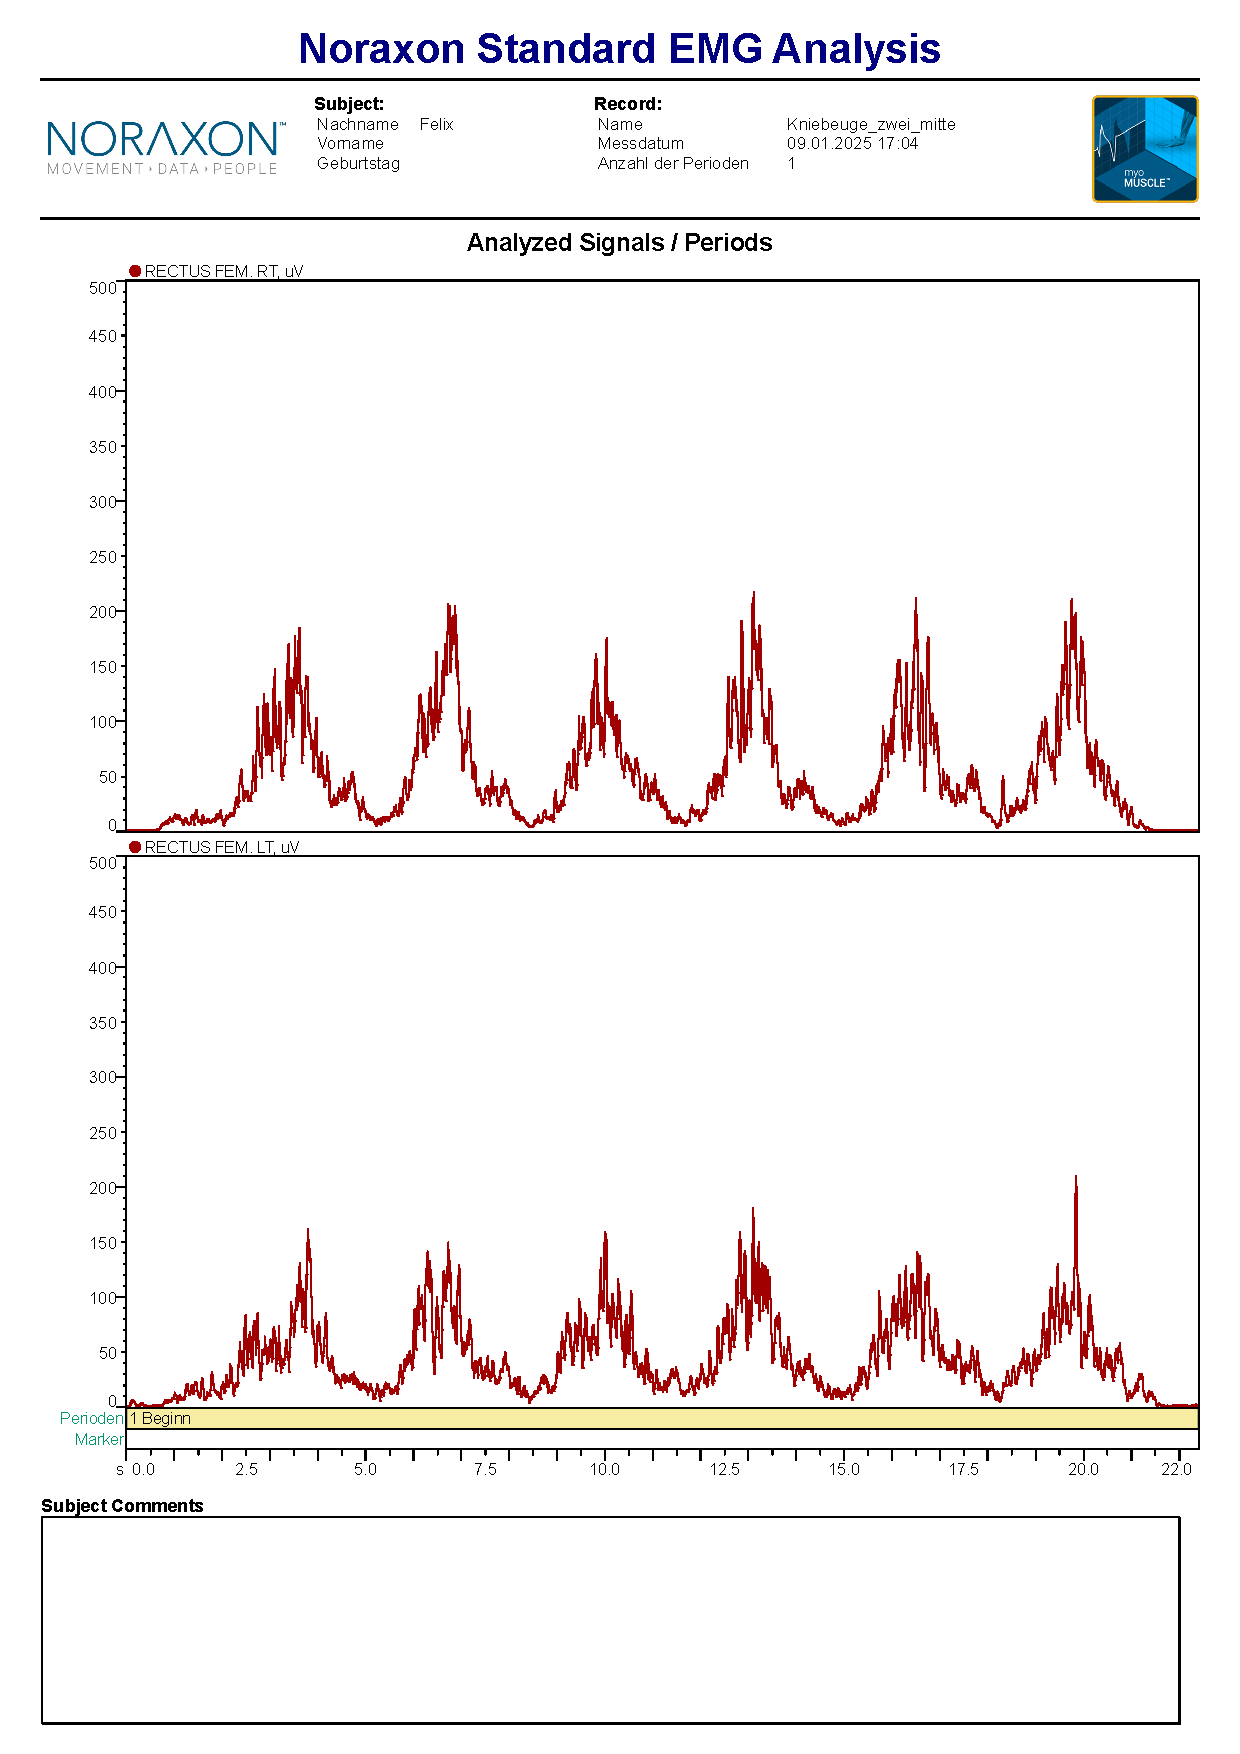
\includegraphics[width=.9\textwidth]{img/pdfs/Felix_2_mitte.pdf}
\clearpage

\subsection*{Felix Innen - Nachher}
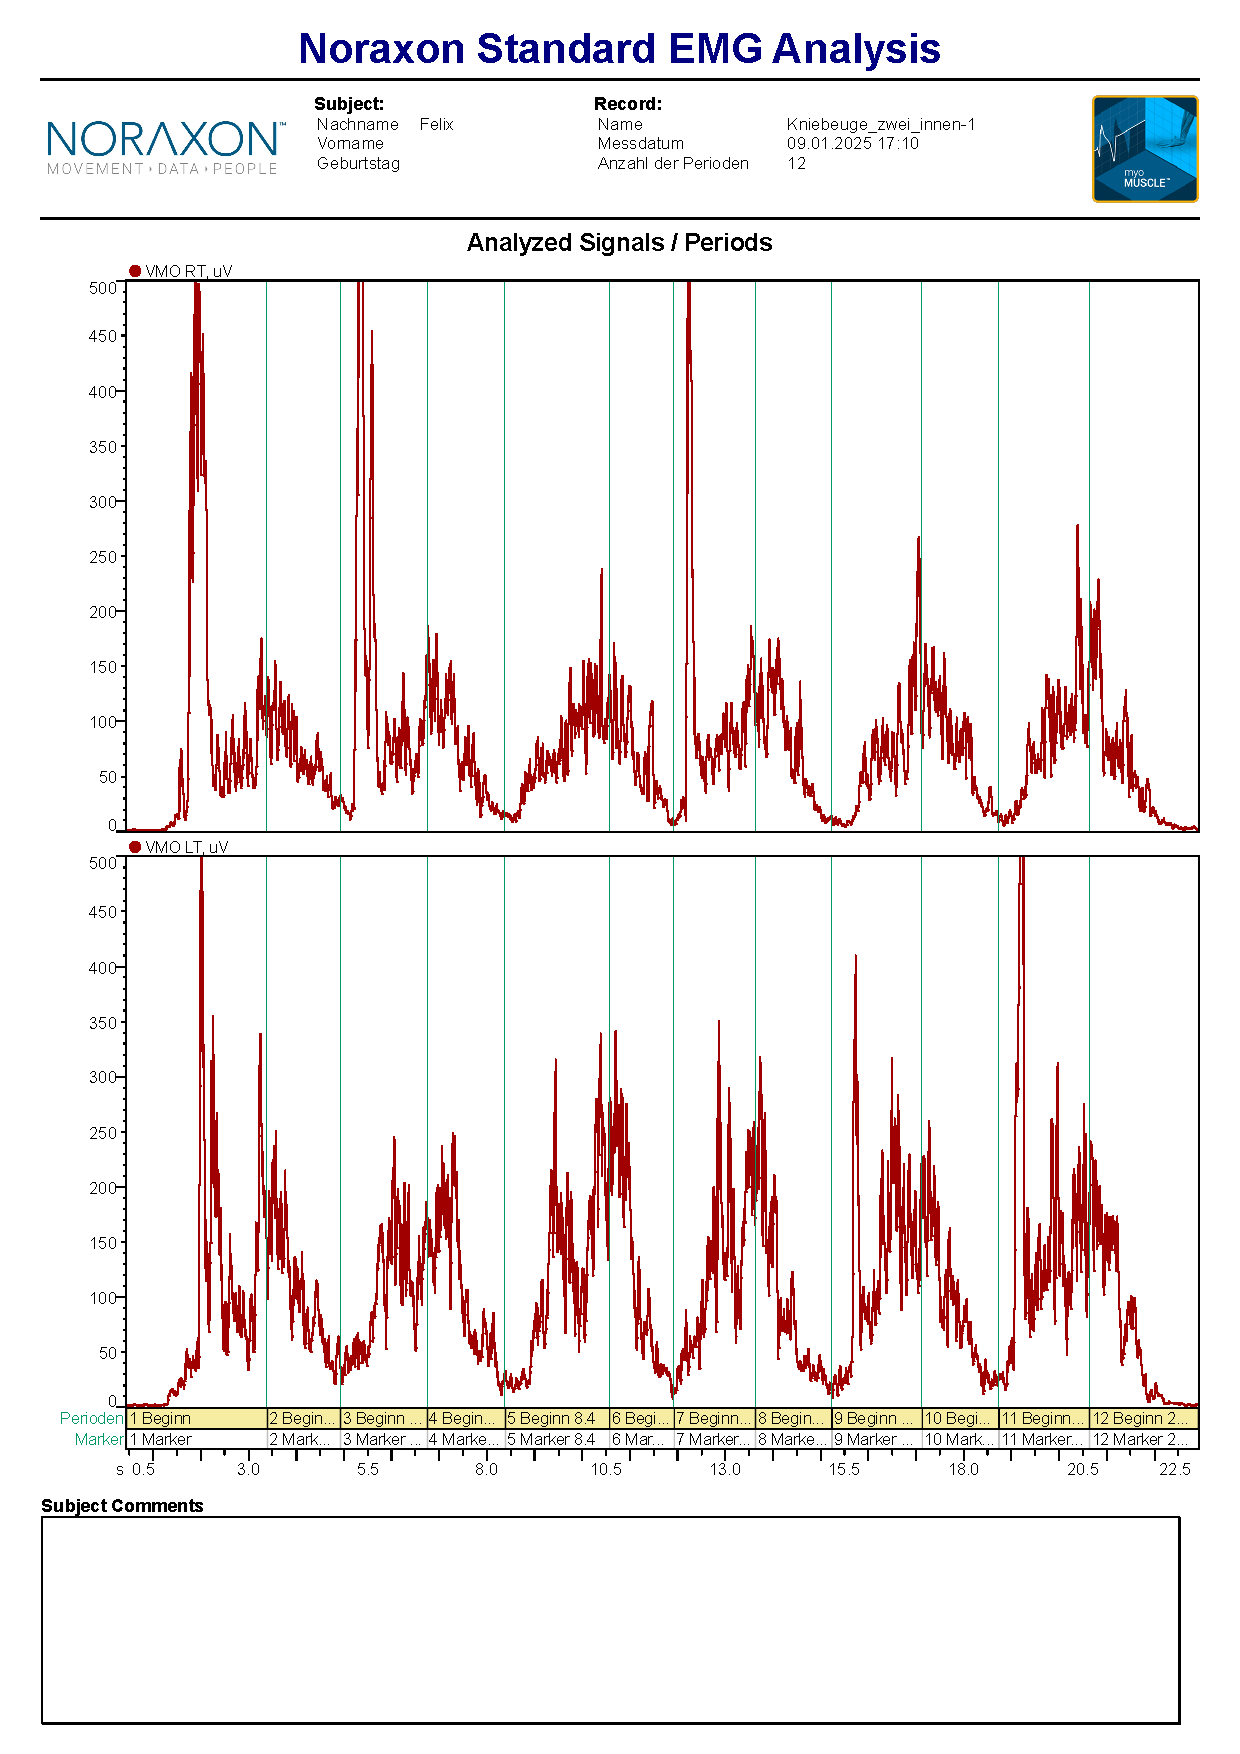
\includegraphics[width=.9\textwidth]{img/pdfs/Felix_2_innen.pdf}
\clearpage

\subsection*{Giorgio Außen - Vorher}
\includegraphics[width=.9\textwidth]{img/pdfs/Gio_Außen_1.pdf}
\clearpage

\subsection*{Giorgio Mitte - Vorher}
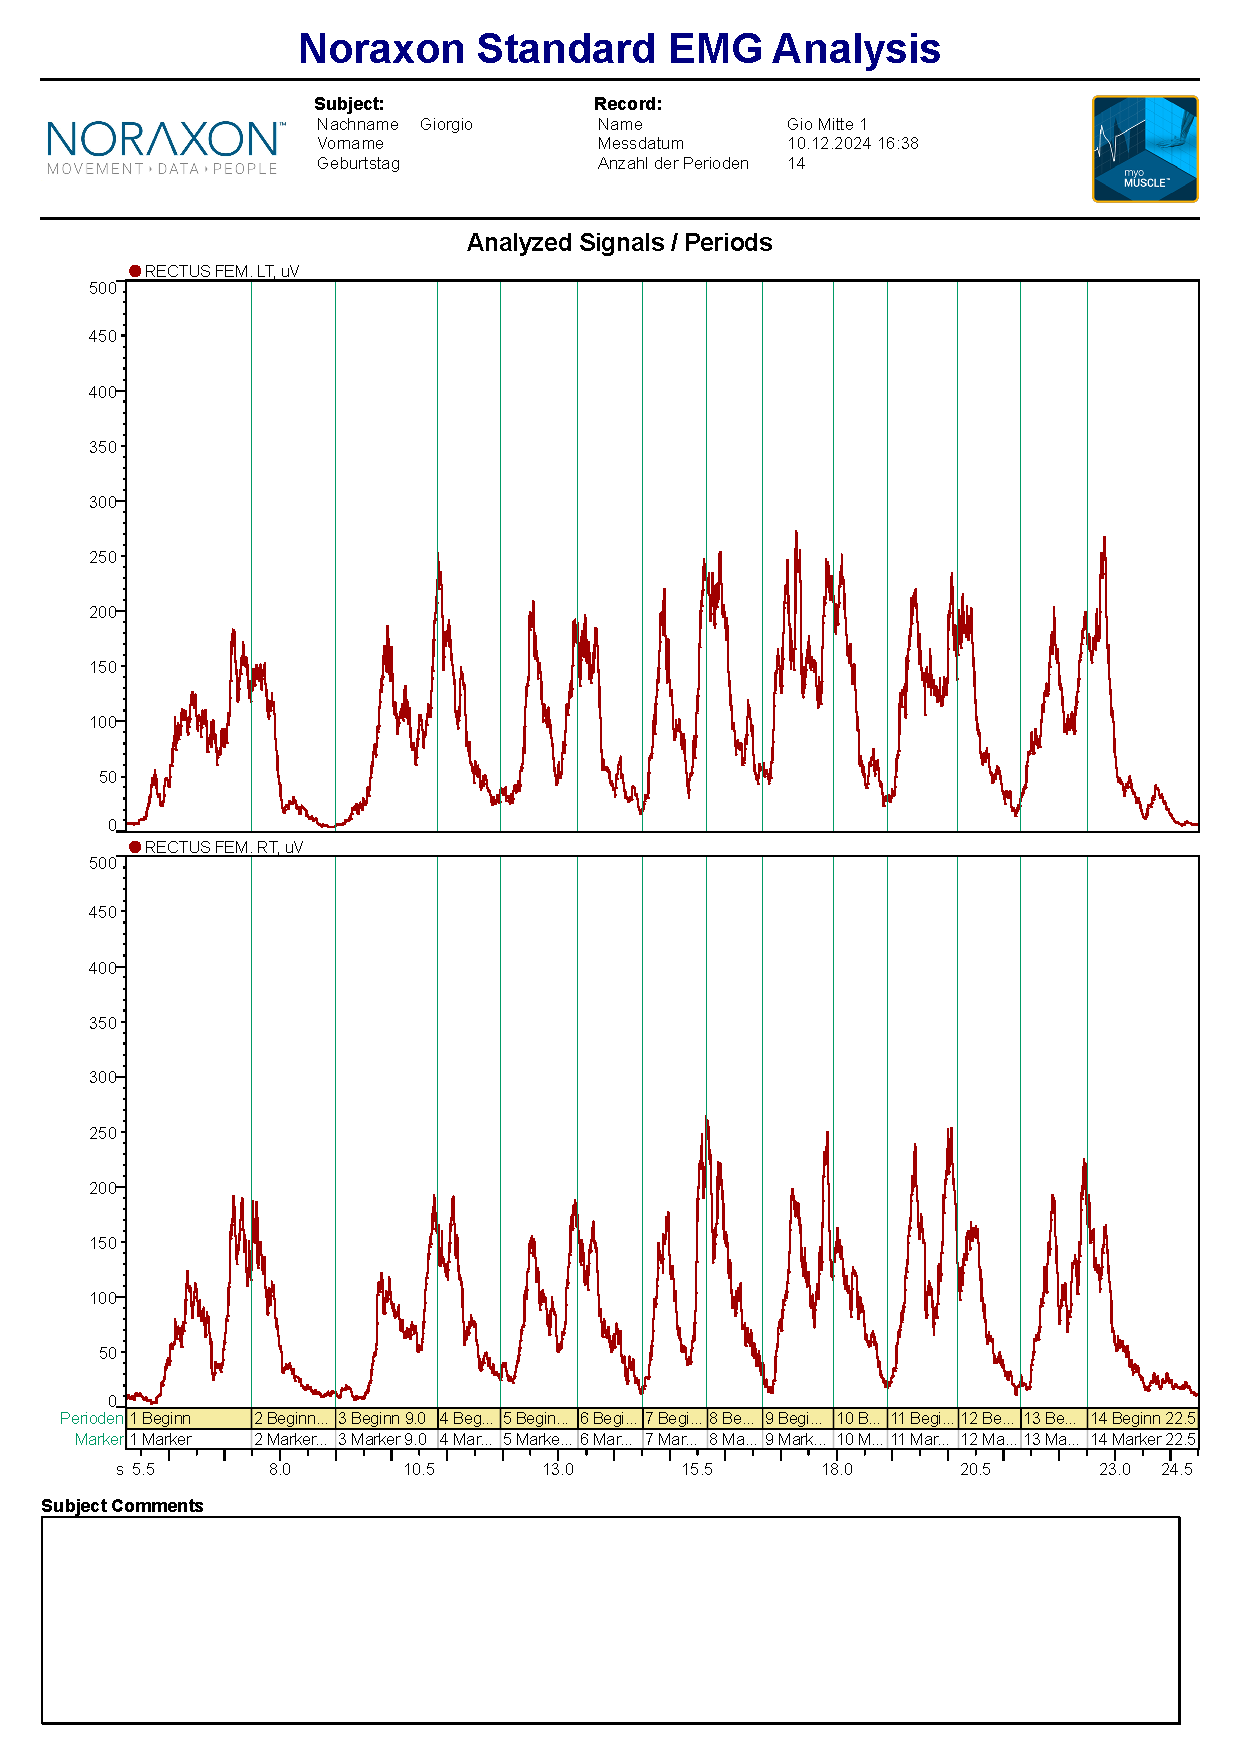
\includegraphics[width=.9\textwidth]{img/pdfs/Gio_Mitte_1.pdf}
\clearpage

\subsection*{Giorgio Innen - Vorher}
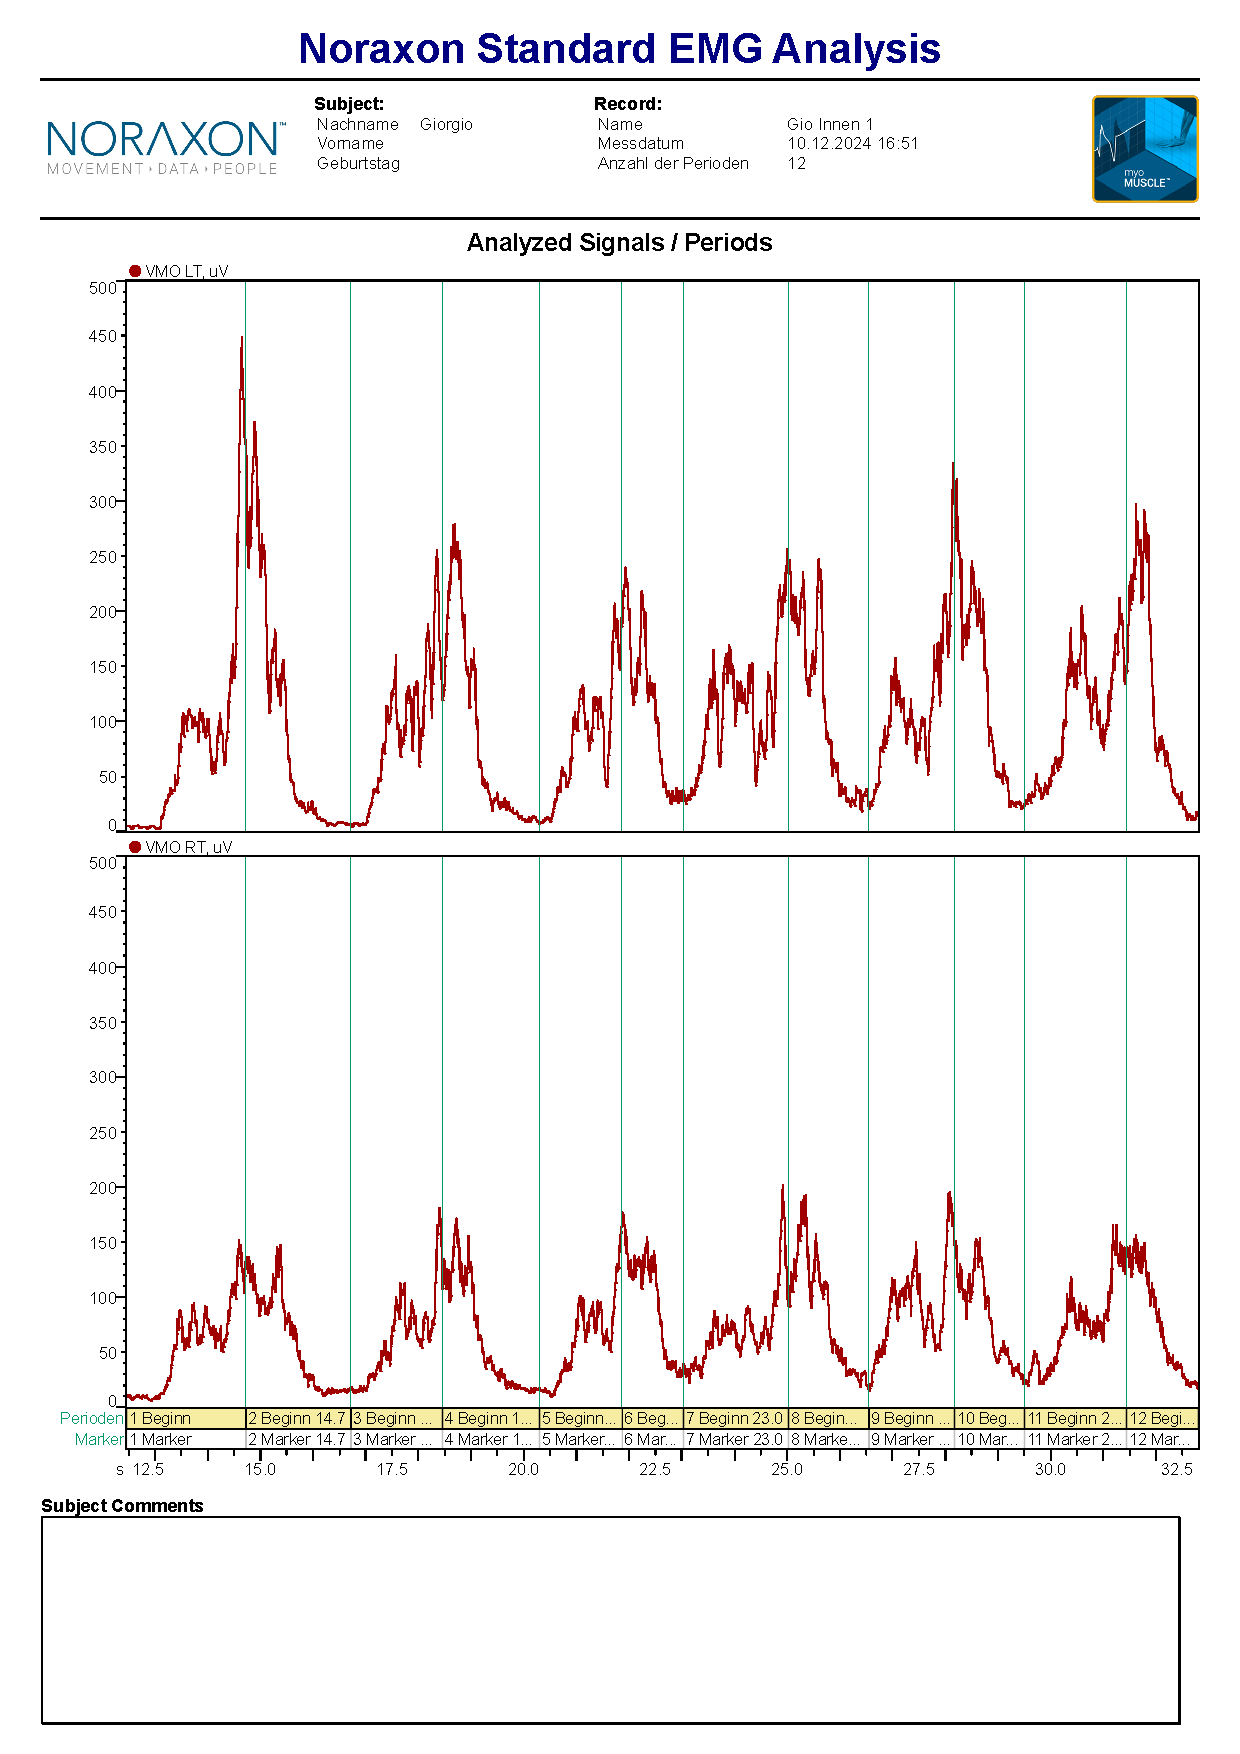
\includegraphics[width=.9\textwidth]{img/pdfs/Gio_Innen_1.pdf}
\clearpage

\subsection*{Giorgio Außen - Nachher}
\includegraphics[width=.9\textwidth]{img/pdfs/Gio_2_außen.pdf}
\clearpage

\subsection*{Giorgio Mitte - Nachher}
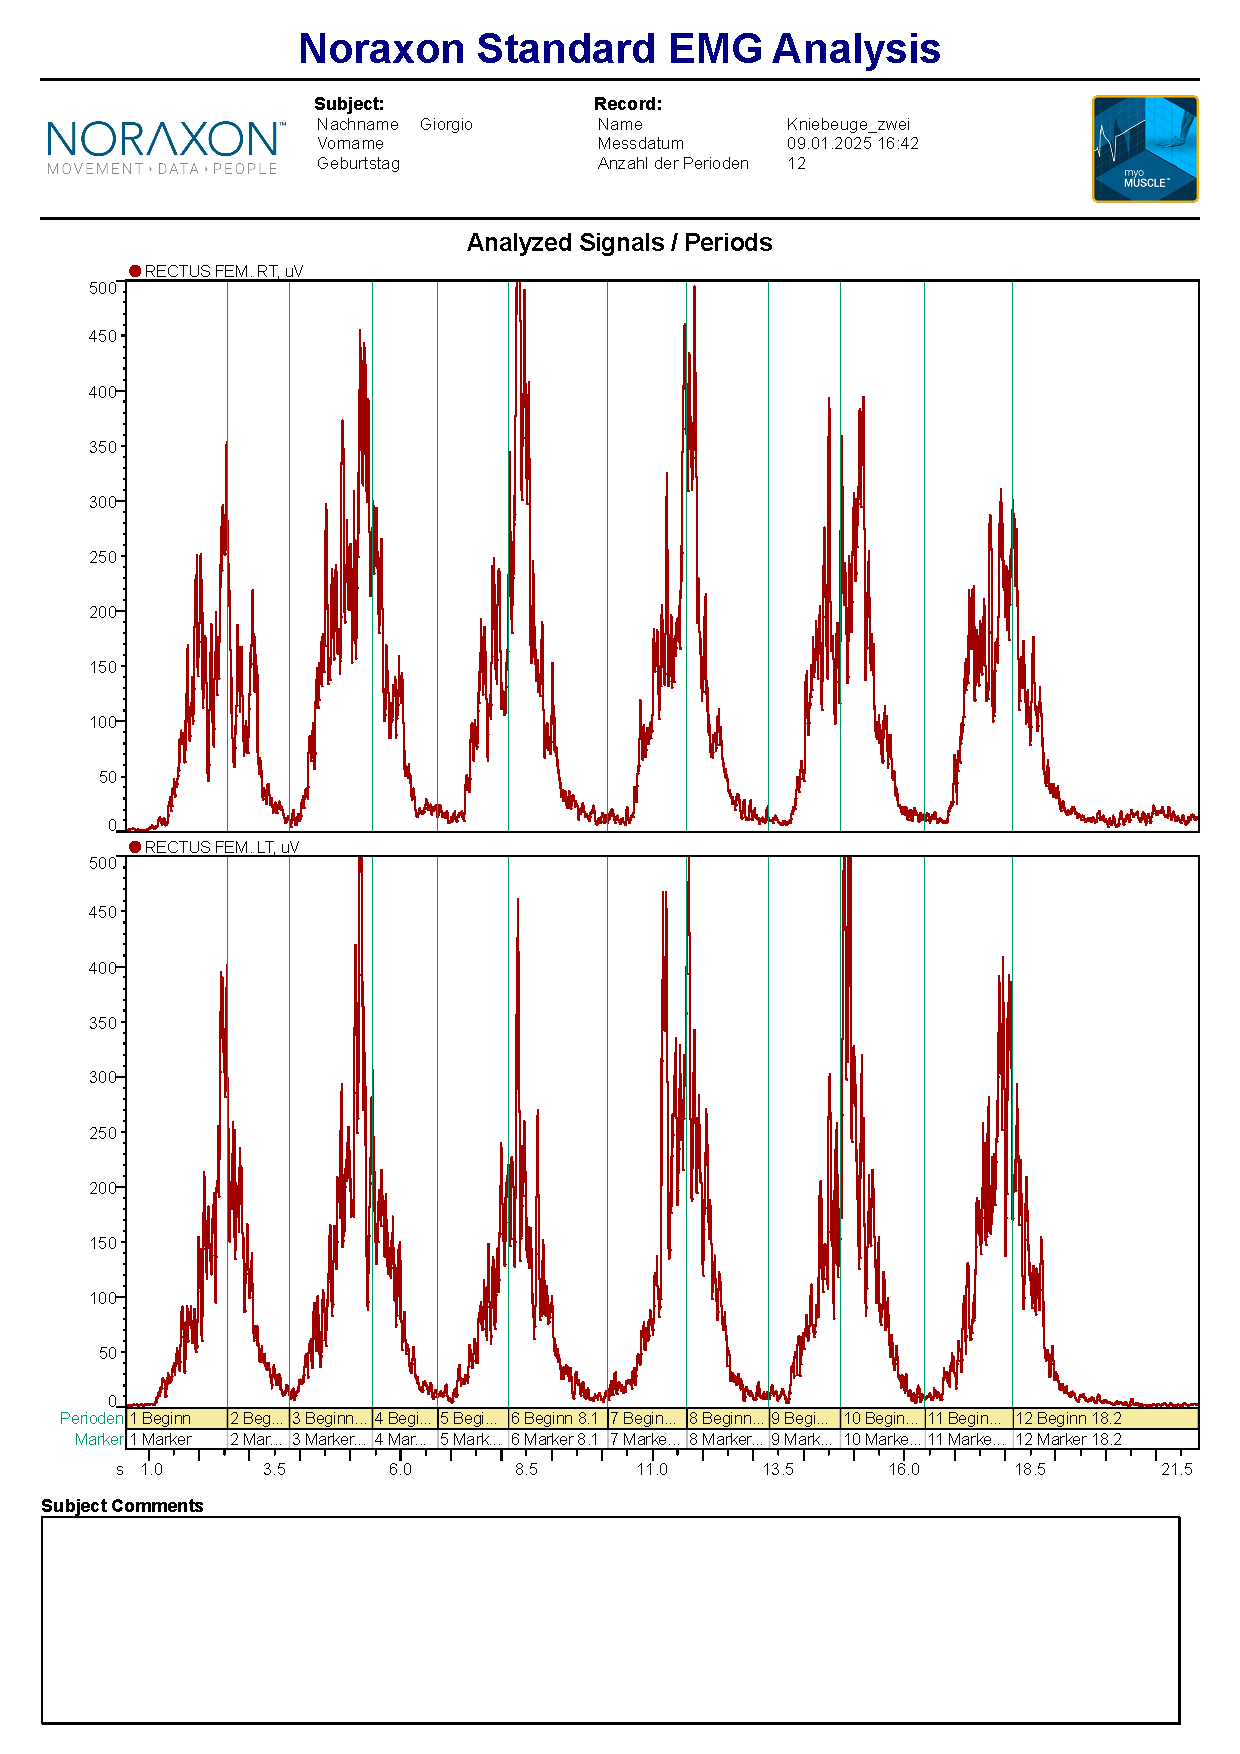
\includegraphics[width=.9\textwidth]{img/pdfs/Gio_2_mitte.pdf}
\clearpage

\subsection*{Giorgio Innen - Nachher}
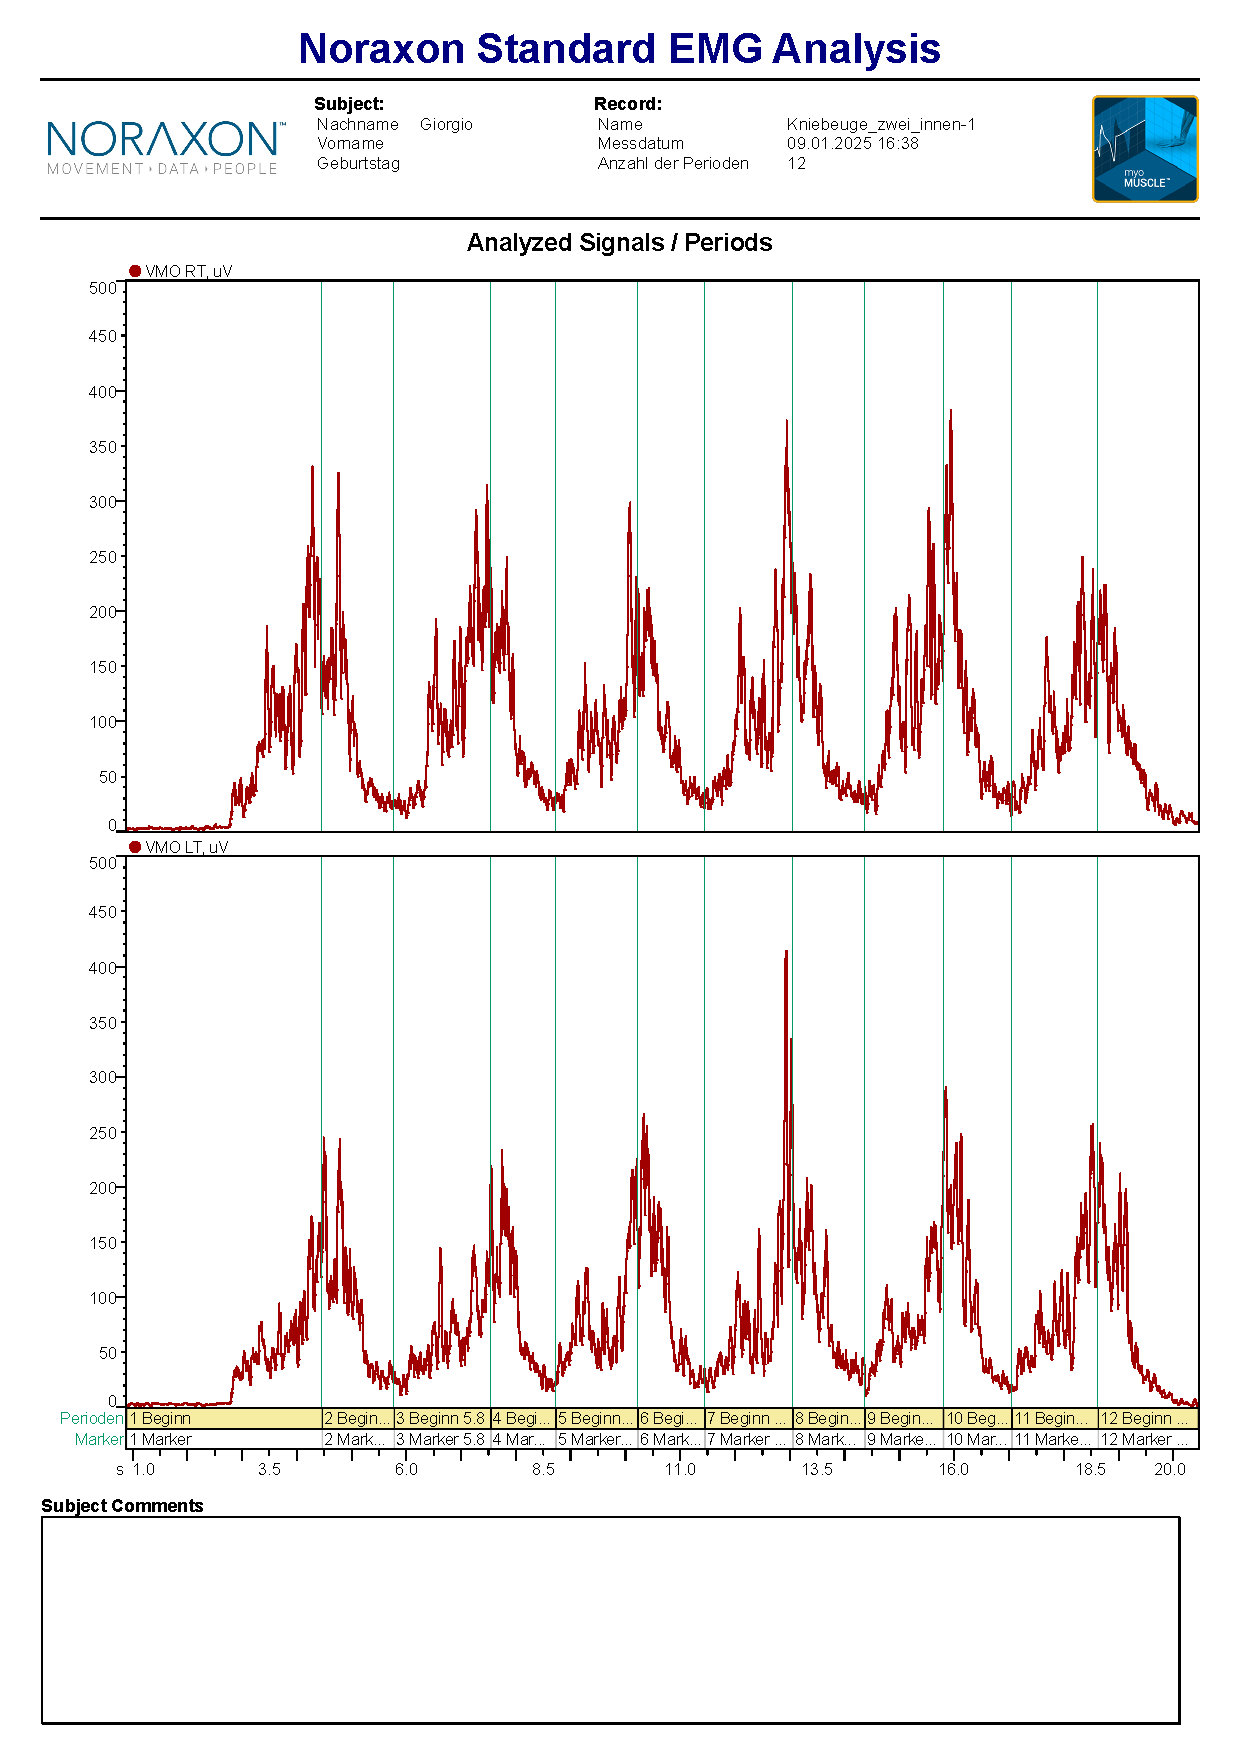
\includegraphics[width=.9\textwidth]{img/pdfs/Gio_2_innen.pdf}
\clearpage

\subsection*{Max Außen - Vorher}
\includegraphics[width=.9\textwidth]{img/pdfs/Maxi_Außen_1.pdf}
\clearpage

\subsection*{Max Mitte - Vorher}
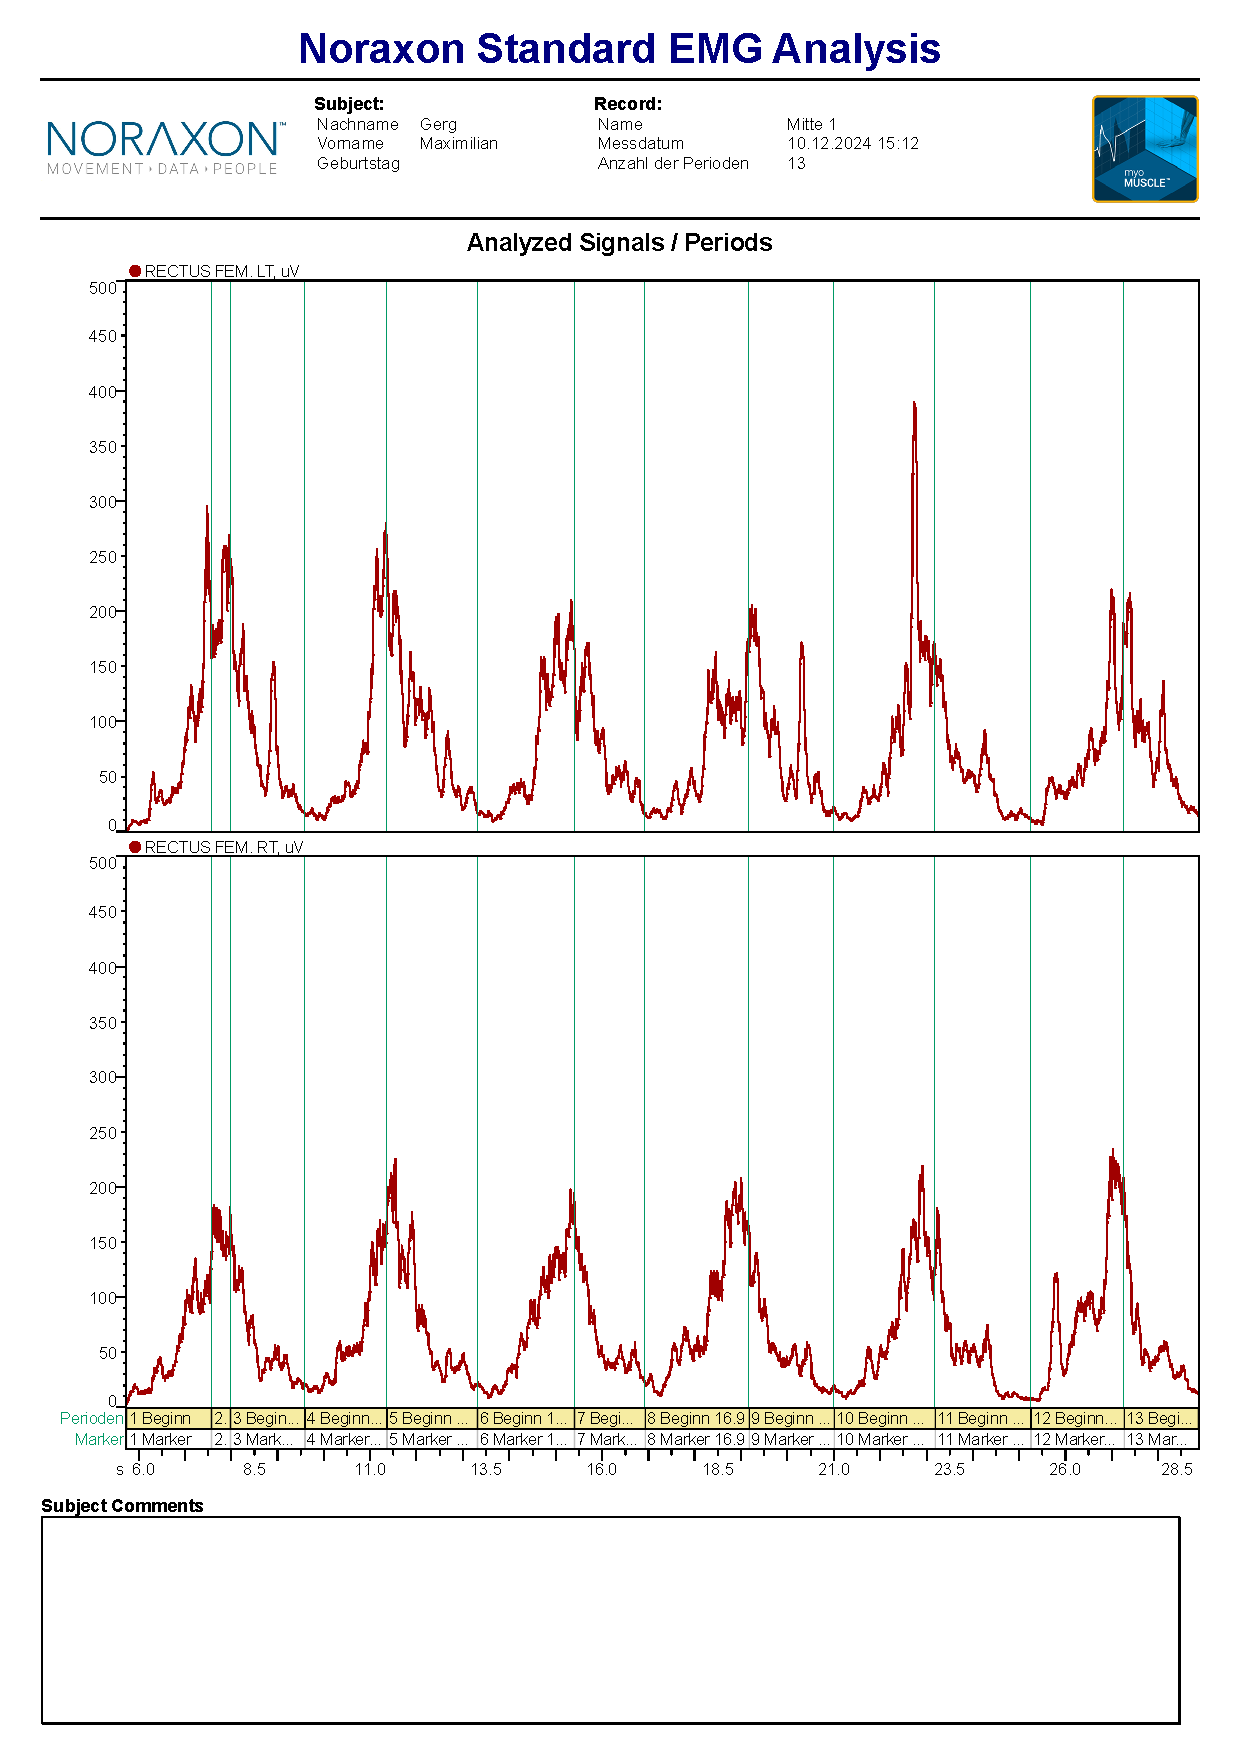
\includegraphics[width=.9\textwidth]{img/pdfs/Maxi_Mitte_1.pdf}
\clearpage

\subsection*{Max Innen - Vorher}
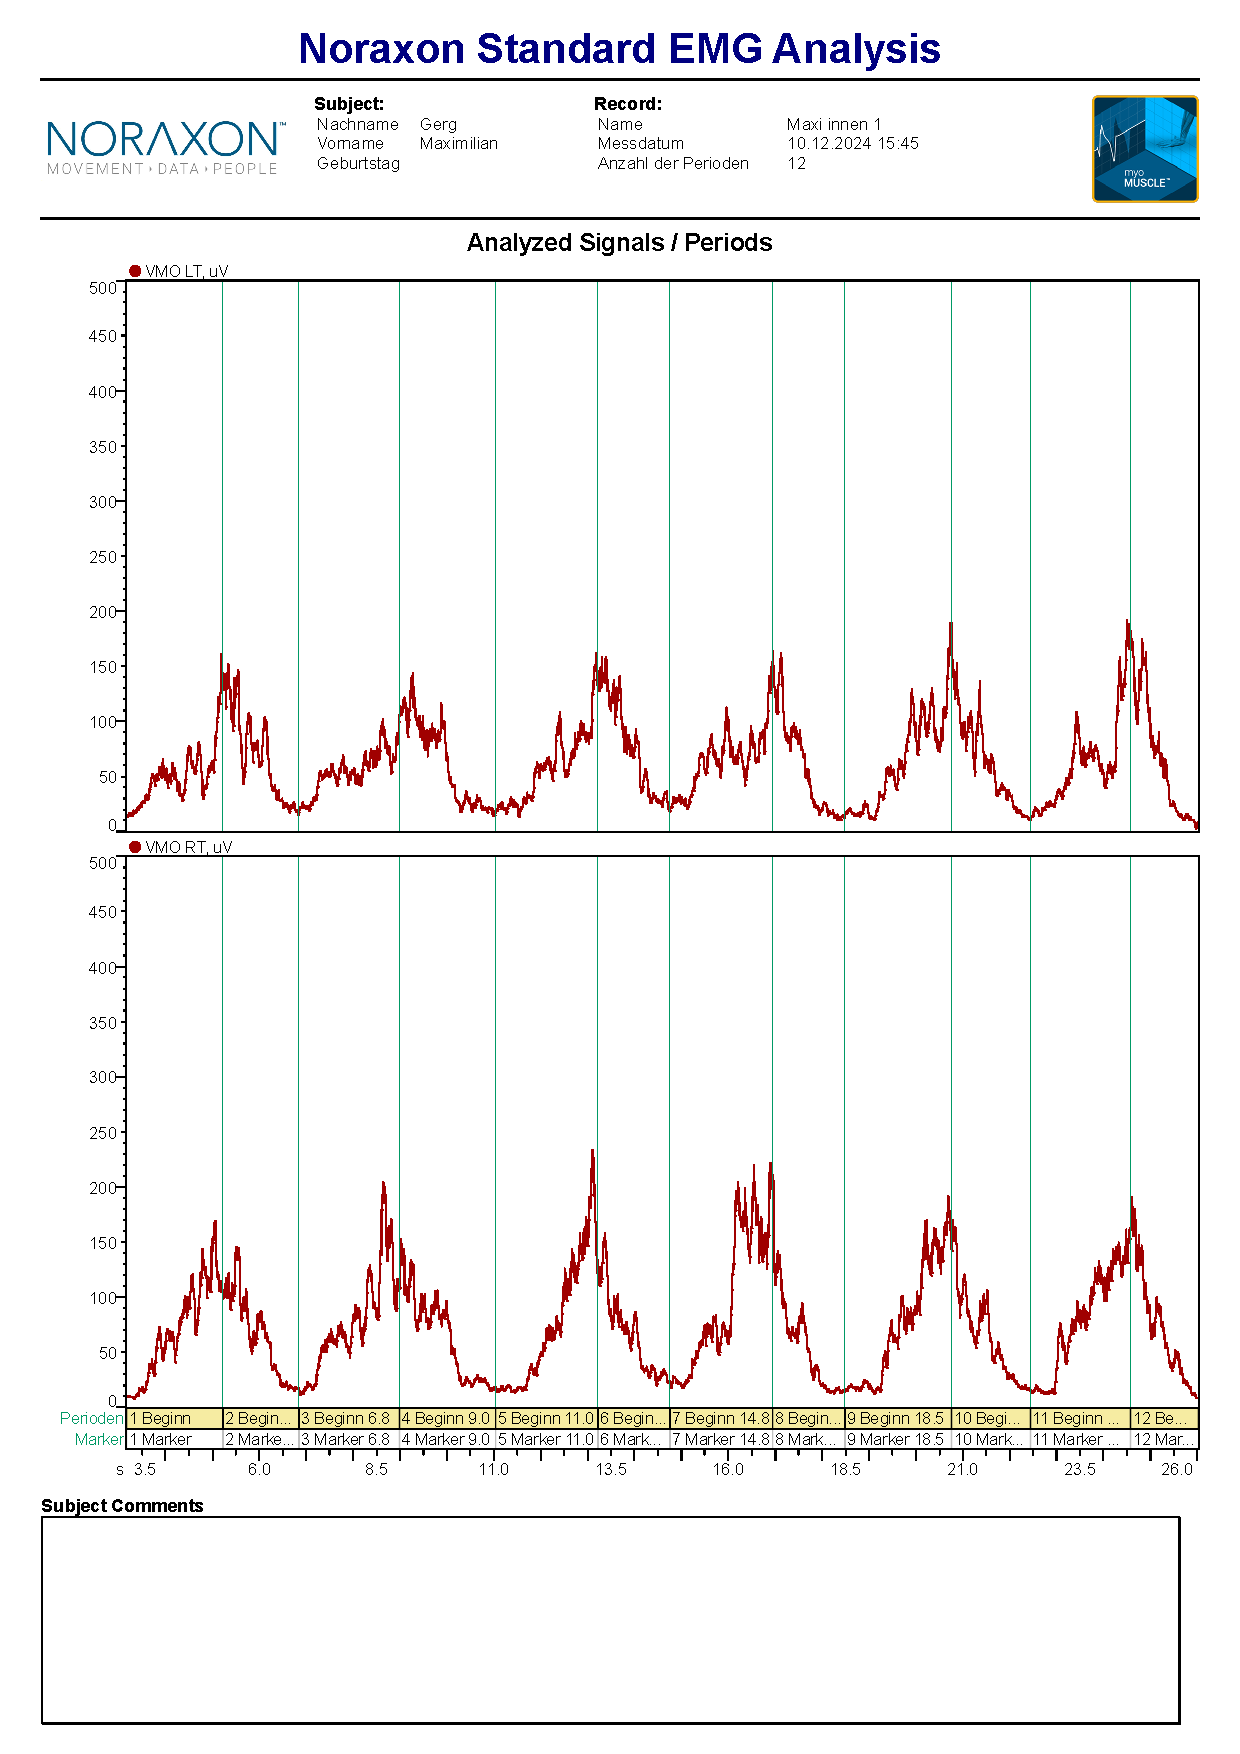
\includegraphics[width=.9\textwidth]{img/pdfs/Maxi_Innen_1.pdf}
\clearpage

\subsection*{Max Außen - Nachher}
\includegraphics[width=.9\textwidth]{img/pdfs/Max_2_außen.pdf}
\clearpage

\subsection*{Max Mitte - Nachher}
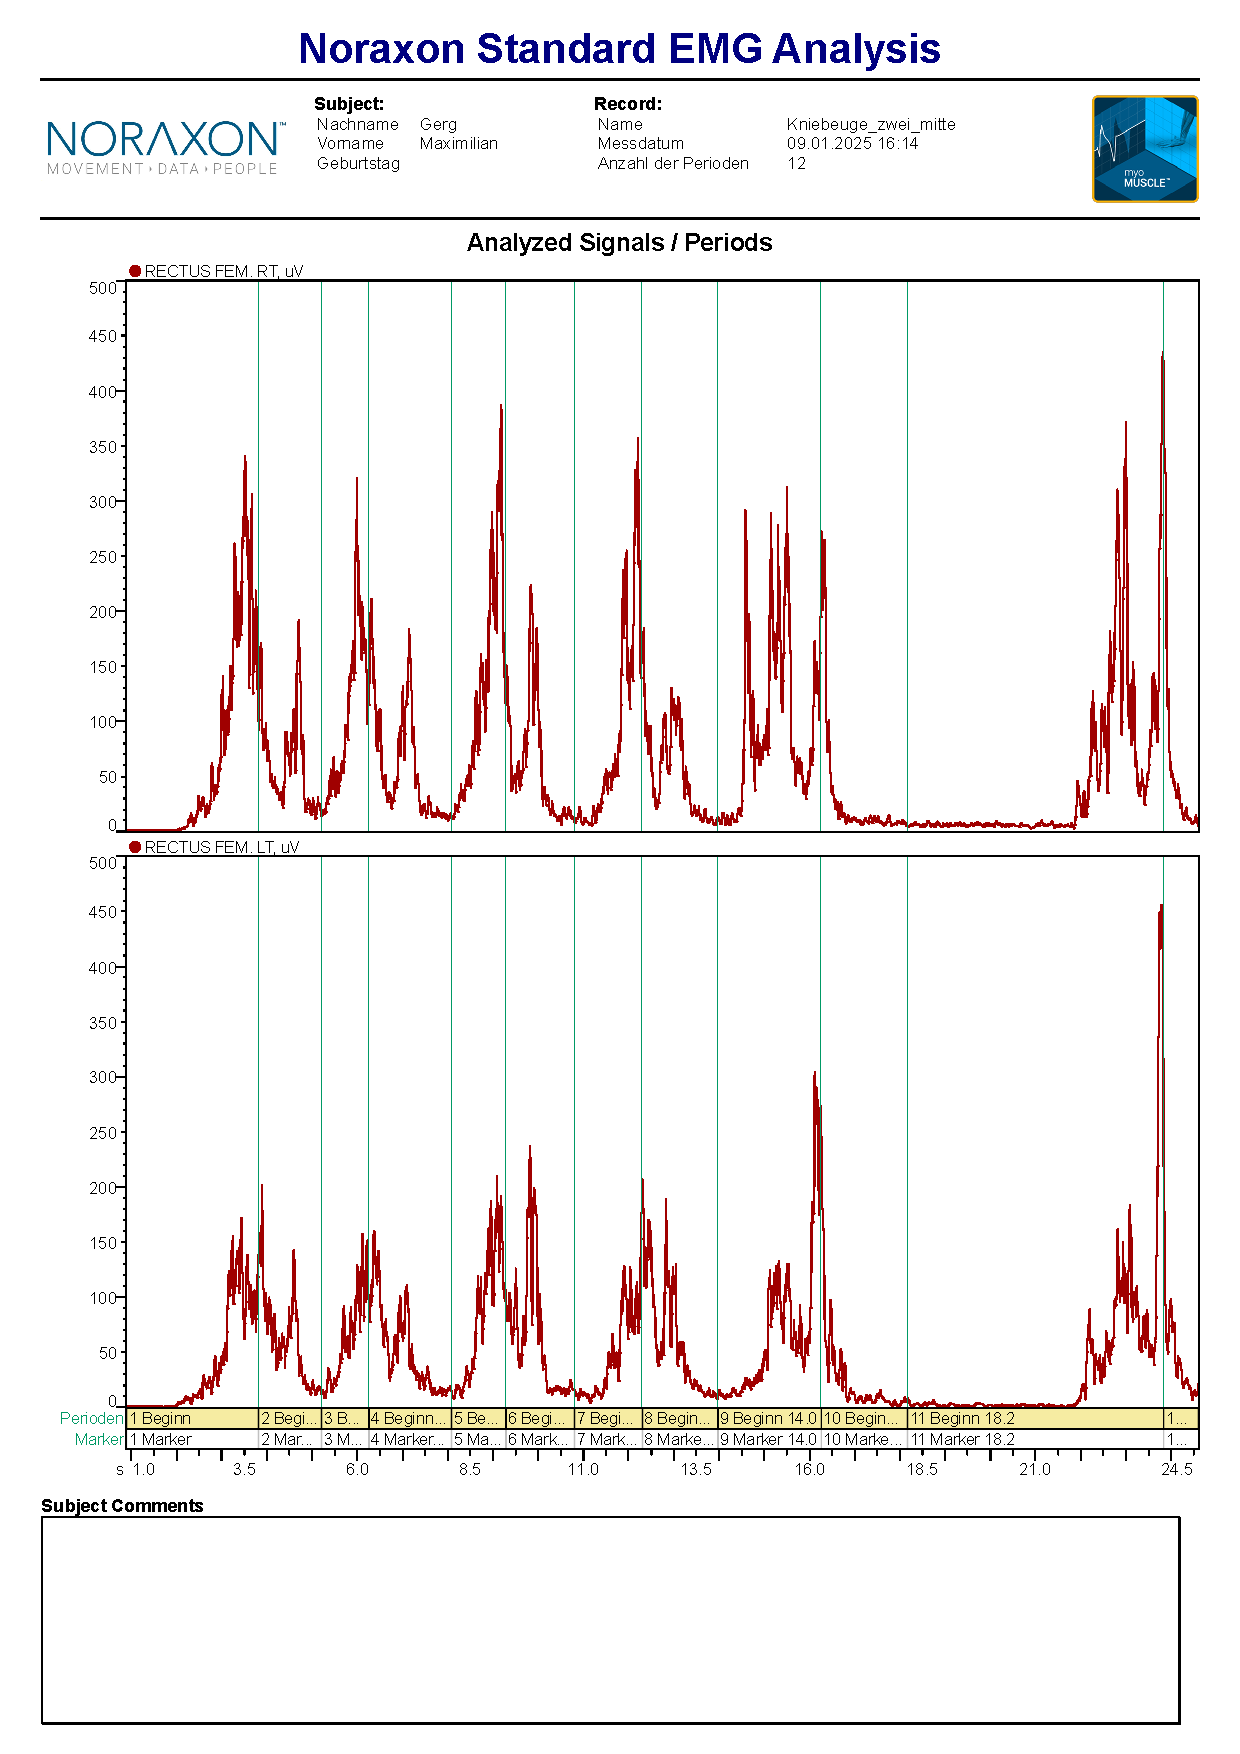
\includegraphics[width=.9\textwidth]{img/pdfs/Max_2_mitte.pdf}
\clearpage

\subsection*{Max Innen - Nachher}
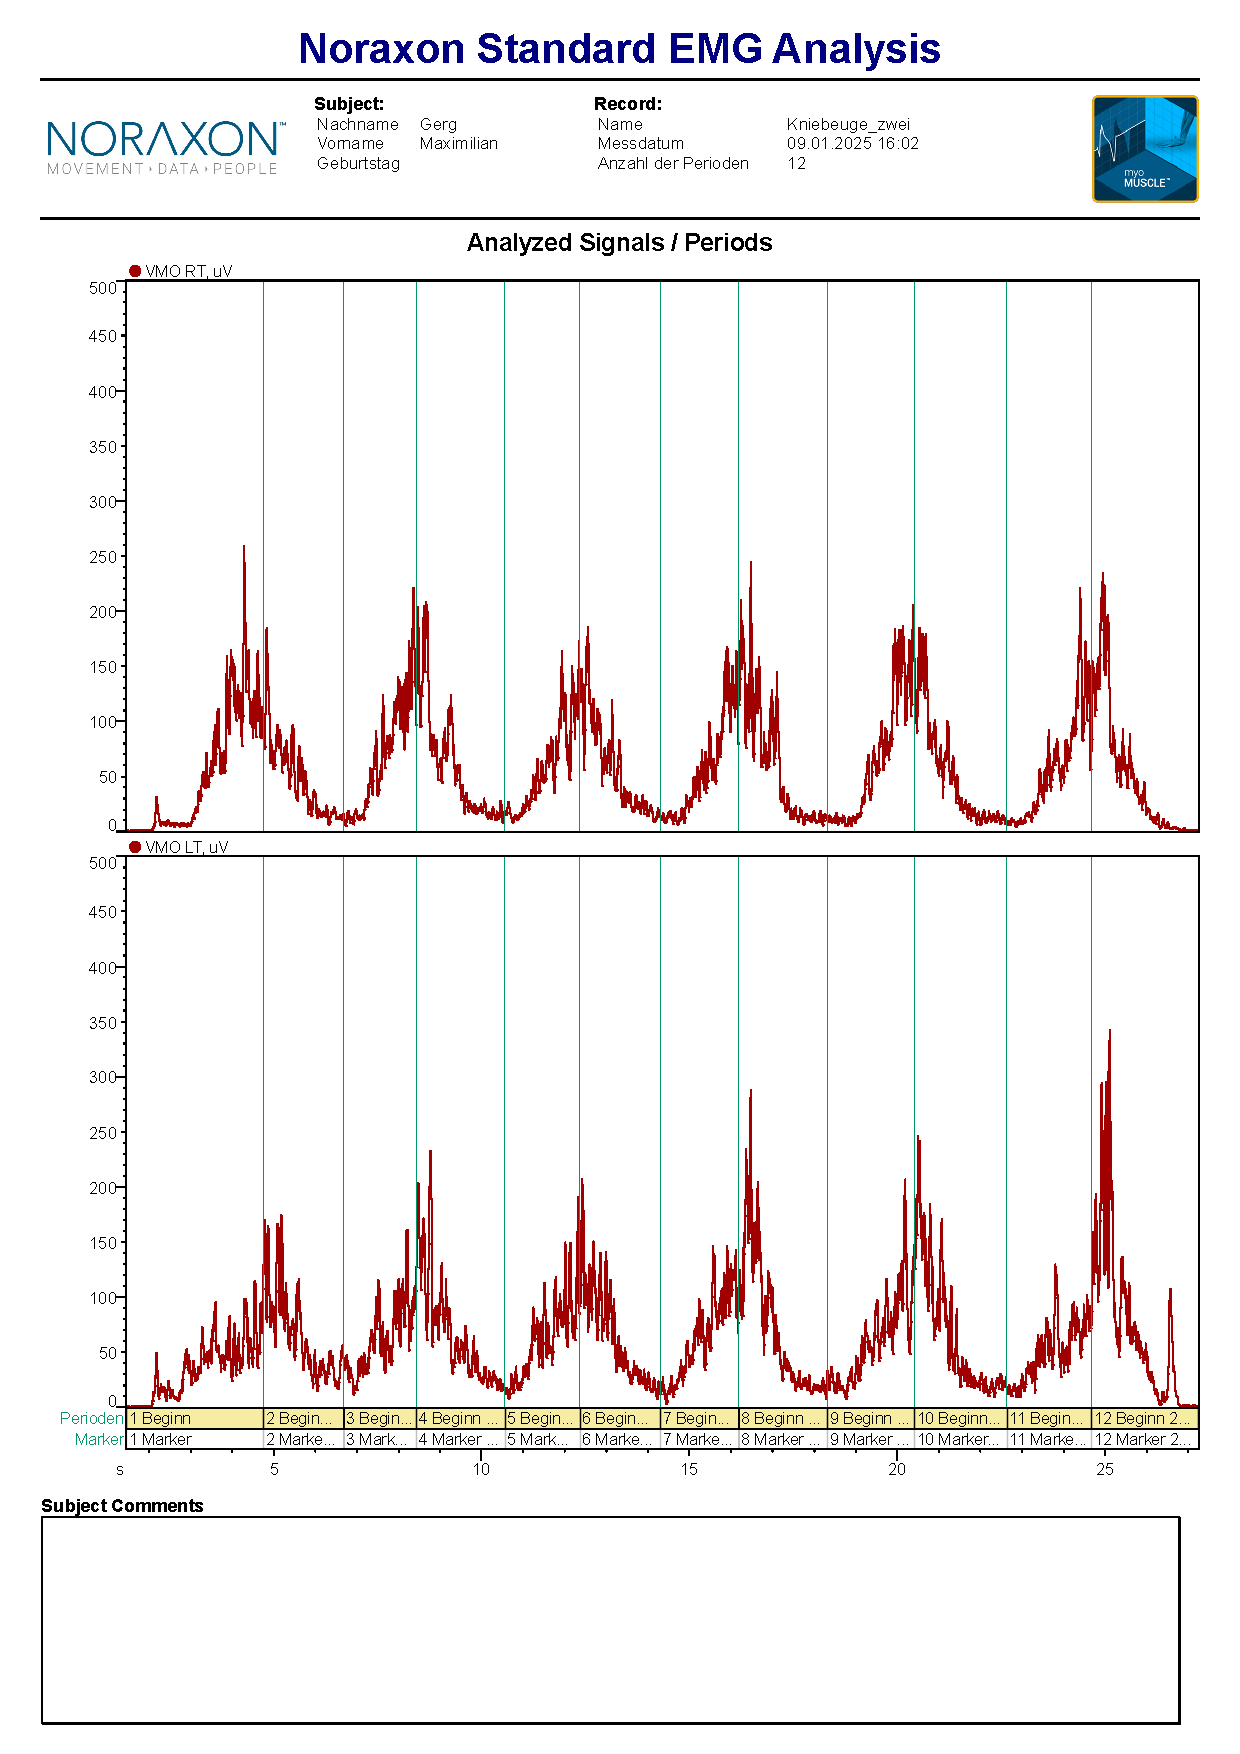
\includegraphics[width=.9\textwidth]{img/pdfs/Max_2_innen.pdf}
\clearpage







% Add more \includepdf lines as needed for additional PDFs


\end{document}
